% ------------------------------------------------------------------------------
% FORMATVORLAGE DOKU/ BEDIENUNGSANLEITUNG
% ------------------------------------------------------------------------------

% DOKUMENTENKOPF ---------------------------------------------------------------
%   Diese Vorlage basiert auf "scrreprt" aus dem koma-script.
% ------------------------------------------------------------------------------
\documentclass[
    11pt,    % Schriftgr��e
    DIV10,
    ngerman, % f�r Umlaute, Silbentrennung etc.
    a4paper, % Papierformat
    oneside, % einseitiges Dokument
    titlepage, % es wird eine Titelseite verwendet
    parskip=half, % Abstand zwischen Abs�tzen (halbe Zeile)
    headings=normal, % Gr��e der �berschriften verkleinern
    listof=totoc, % Verzeichnisse im Inhaltsverzeichnis auff�hren
    bibliography=totoc, % Literaturverzeichnis im Inhaltsverzeichnis auff�hren
    index=totoc, % Index im Inhaltsverzeichnis auff�hren
    captions=tableheading, % Beschriftung von Tabellen unterhalb ausgeben
    final % Status des Dokuments (final/draft)
]{scrreprt}

% globale Definitionen -----------------------------------------------------------
%   Informationen �ber das Dokument, wie z.B. Titel, Autor, Datum 
%   werden in der Datei globale_Definitionen.tex definiert und k�nnen danach global
%   verwendet werden.
% ------------------------------------------------------------------------------
% Meta-Informationen -----------------------------------------------------------
%   Definition von globalen Parametern, die im gesamten Dokument verwendet
%   werden k�nnen (z.B auf dem Deckblatt etc.).
%
%   ACHTUNG: Wenn die Texte Umlaute oder ein Esszet enthalten, muss der folgende
%            Befehl bereits an dieser Stelle aktiviert werden:
%            \usepackage[latin1]{inputenc}
% ------------------------------------------------------------------------------
\newcommand{\titel}{Mediaplayer {\Bezeichnung} f�r den Raspberry Pi Modell B+}
\newcommand{\untertitel}{}%{TODO: und hier kommt der Untertitel}
\newcommand{\Bezeichnung}{YAMuPlay}
\newcommand{\BezeichnungLang}{Yet Another Music Player}
\newcommand{\Version}{V0.1}
\newcommand{\Dokumentart}{D O K U M E N T A T I O N}
\newcommand{\autor}{schlizb�da}
\newcommand{\jahr}{2016}
\newcommand{\bauwong}{Bauwong n.e.V.}
\newcommand{\logo}{bauwong.pdf}

\newcommand{\WandermontageDoppelt}{\textit{10125 Montagelinie HMI}}
\newcommand{\DienststelleME}{I IA CE CP MF GWA ME 2 M-720}
\newcommand{\SimaticNetSoftware}{SIMATIC NET PC-Software V12+SP2}

% verwendete Hardware
\newcommand{\RPi}{Raspberry Pi}
\newcommand{\Ligawo}{Ligawo 6518725 HDMI Extractor}
% http://www.amazon.de/Ligawo-%C2%AE-HDMI-Audio-Extractor/dp/B00CAQN0CM/ref=cm_cr_pr_product_top?ie=UTF8&tag=httpwwwforumr-21  Variante C: RCA (Cinch)
% http://www.amazon.de/dp/B00ADJIVB8 (RPi-Forum)

% verwendete Software
\newcommand{\matchboxKeyboard}{matchbox-keyboard}



%Steuerelemente von Software:
\newcommand{\prompt}[1]{\Code{\textit{#1}}}
\newcommand{\filenam}[1]{\Code{#1}}

\newcommand{\button}[1]{\Code{[{#1}]}}
\newcommand{\menuitem}[1]{\textbf{\textit{"{#1}"}}}
\newcommand{\checkbox}[1]{\textbf{\textit{"{#1}"}}}

\newcommand{\Verein}[1]{\textit{#1}}


%Smileys:
\newcommand{\smiley}[1]{\includegraphics[width=0.3cm]{Bilder/smileys/{#1}}}


% ben�tigte Packages -----------------------------------------------------------
%   LaTeX-Packages, die ben�tigt werden, sind in die Datei Packages.tex
%   "ausgelagert", um diese Vorlage m�glichst �bersichtlich zu halten.
% ------------------------------------------------------------------------------
% Anpassung des Seitenlayouts --------------------------------------------------
%   siehe Seitenstil.tex
% ------------------------------------------------------------------------------
\usepackage[
    automark, % Kapitelangaben in Kopfzeile automatisch erstellen
    headsepline, % Trennlinie unter Kopfzeile
    ilines % Trennlinie linksb�ndig ausrichten
]{scrpage2}

% Anpassung an Landessprache ---------------------------------------------------
\usepackage[ngerman]{babel}

% Umlaute ----------------------------------------------------------------------
%   Umlaute/Sonderzeichen wie ���� direkt im Quelltext verwenden (CodePage).
%   Erlaubt automatische Trennung von Worten mit Umlauten.
% ------------------------------------------------------------------------------
\usepackage[latin1]{inputenc}
%\usepackage[utf8]{inputenc}
\usepackage[T1]{fontenc}
\usepackage{textcomp} % Euro-Zeichen,Copyright etc.

% Schrift ----------------------------------------------------------------------
\usepackage{lmodern} % bessere Fonts
\usepackage{relsize} % Schriftgr��e relativ festlegen

% Grafiken ---------------------------------------------------------------------
% Einbinden von JPG-Grafiken erm�glichen
\usepackage[dvips,final]{graphicx}
% hier liegen die Bilder des Dokuments
\graphicspath{{Bilder/}}

% Befehle aus AMSTeX f�r mathematische Symbole z.B. \boldsymbol \mathbb --------
\usepackage{amsmath,amsfonts}

% f�r Index-Ausgabe mit \printindex --------------------------------------------
\usepackage{makeidx}

% Einfache Definition der Zeilenabst�nde und Seitenr�nder etc. -----------------
\usepackage{setspace}
\usepackage{geometry}

% ------------------------------------------------------------------------------
% --- Abk�rzungsverzeichnis ----------------------------------------------------
% ------------------------------------------------------------------------------
%   Symbolverzeichnisse bequem erstellen. Beruht auf MakeIndex:
%     makeindex.exe %Name%.nlo -s nomencl.ist -o %Name%.nls
%   erzeugt dann das Verzeichnis. Dieser Befehl kann z.B. im TeXnicCenter
%   als Postprozessor eingetragen werden, damit er nicht st�ndig manuell
%   ausgef�hrt werden muss.
%   Die Definitionen sind ausgegliedert in die Datei "Glossar.tex".
% ------------------------------------------------------------------------------
\usepackage[intoc]{nomencl}
\let\abbrev\nomenclature
\renewcommand{\nomname}{Abk�rzungsverzeichnis}
\setlength{\nomlabelwidth}{.25\hsize}
\renewcommand{\nomlabel}[1]{#1 \dotfill}
\setlength{\nomitemsep}{-\parsep}

\usepackage{acronym}


% zum Umflie�en von Bildern ----------------------------------------------------
\usepackage{floatflt}

% ------------------------------------------------------------------------------
% --- Listings zum einbinden von CODE ------------------------------------------
% ------------------------------------------------------------------------------
\usepackage{listings}
\usepackage[table]{xcolor} 
% Farben f�r listenings definieren! alternativ: {RGB}{0-255,0-255.0-255}
\definecolor{hellgelb}{rgb}{1,1,0.9}			     
\definecolor{colKeys}{rgb}{0,0,1}
\definecolor{colIdentifier}{rgb}{0,0,0}
\definecolor{colComments}{rgb}{0,0.5,0.1} 
\definecolor{colString}{rgb}{1,0,0}
\lstset{
    float=hbp,
    basicstyle=\ttfamily\color{black}\small\smaller, % the size of the fontsthat are used for the code 
    identifierstyle=\color{colIdentifier},
    keywordstyle=\color{colKeys},
    stringstyle=\color{colString},
    commentstyle=\color{colComments},
    columns=flexible,
    tabsize=3,
    %frame=single,                     % add frame arround the code
    extendedchars=true,
    showspaces=false,
    showstringspaces=false,
    numbers=left,                      % where to put the line numbers
    numberstyle=\tiny,                % fontsize for line
    stepnumber= 1,                     % stepnumber between line-numbers
    breaklines=true,                   % sets automatic line breaking
    captionpos=b,                      % sets caption position to bottom
    backgroundcolor=\color{hellgelb},
    breakautoindent=true,
    }

% URL verlinken, lange URLs umbrechen etc. -------------------------------------
\usepackage{url}

% wichtig f�r korrekte Zitierweise ---------------------------------------------
\usepackage[numbers]{natbib}  % [square] to [numbers] jetzt gehen versch. stile

% ------------------------------------------------------------------------------
% --- PDF Optionen -------------------------------------------------------------
% ------------------------------------------------------------------------------
\definecolor{darkblue}{rgb}{0,0,0.5} % def. Farbe f�r PDF Verlinkungen
\usepackage[
    bookmarks,
    bookmarksopen=true,
    colorlinks=true,
% diese Farbdefinitionen zeichnen Links im PDF farblich aus
    linkcolor=darkblue,% einfache interne Verkn�pfungen
    anchorcolor=black,% Ankertext
    citecolor=blue,   % Verweise auf Literaturverzeichniseintr�ge im Text
    filecolor=magenta,% Verkn�pfungen, die lokale Dateien �ffnen
    menucolor=red,    % Acrobat-Men�punkte
    urlcolor=cyan, 
% diese Farbdefinitionen sollten f�r den Druck verwendet werden (alles schwarz)
    %linkcolor=black,  % einfache interne Verkn�pfungen
    %anchorcolor=black,% Ankertext
    %citecolor=black,  % Verweise auf Literaturverzeichniseintr�ge im Text
    %filecolor=black,  % Verkn�pfungen, die lokale Dateien �ffnen
    %menucolor=black,  % Acrobat-Men�punkte
    %urlcolor=black, 
    backref,
    plainpages=false, % zur korrekten Erstellung der Bookmarks
    pdfpagelabels, % zur korrekten Erstellung der Bookmarks
    hypertexnames=false, % zur korrekten Erstellung der Bookmarks
    linktocpage % Seitenzahlen anstatt Text im Inhaltsverzeichnis verlinken
]{hyperref}
% Befehle, die Umlaute ausgeben, f�hren zu Fehlern, wenn sie hyperref als Optionen �bergeben werden
\hypersetup{
    pdftitle={\titel \untertitel},
    pdfauthor={\autor},
    pdfcreator={\autor},
    pdfsubject={\titel \untertitel},
    pdfkeywords={\titel \untertitel},
}

% fortlaufendes Durchnummerieren der Fu�noten ----------------------------------
\usepackage{chngcntr}

% f�r lange Tabellen -----------------------------------------------------------
\usepackage{longtable}
\usepackage{array}
\usepackage{ragged2e}
\usepackage{lscape}

% Spaltendefinition rechtsb�ndig mit definierter Breite ------------------------
\newcolumntype{w}[1]{>{\raggedleft\hspace{0pt}}p{#1}}

% Formatierung von Listen �ndern -----------------------------------------------
\usepackage{paralist}

% bei der Definition eigener Befehle ben�tigt
\usepackage{ifthen}

% definiert u.a. die Befehle \todo und \listoftodos
\usepackage{todonotes}

% sorgt daf�r, dass Leerzeichen hinter parameterlosen Makros nicht als Makroendezeichen interpretiert werden
\usepackage{xspace}

% zur Formatierung der Abbildungsunterschriften (Captions)
\usepackage{caption}
\captionsetup{labelfont=bf,textfont=it} % Abbildung fett, Text kursiv

% zum Einbinden von Messageboxen 
\usepackage[tikz]{bclogo}

% zum Formatieren von Tabellen
\usepackage{booktabs}
\renewcommand{\arraystretch}{1}% Zeilenabstand in einer Tabelle auf 2

% zum Einbinden von PDF Dateien
\usepackage{pdfpages}


% Erstellung eines Index und Abk�rzungsverzeichnisses aktivieren ---------------
\makeindex
\makenomenclature

% Kopf- und Fu�zeilen, Seitenr�nder etc. ---------------------------------------


% Zeilenabstand 1,5 Zeilen -----------------------------------------------------
\onehalfspacing

% ------------------------------------------------------------------------------
% ----------- Seitenr�nder -----------------------------------------------------
% ------------------------------------------------------------------------------

\setlength{\topskip}{\ht\strutbox} % behebt Warnung von geometry
\geometry{paper=a4paper,left=30mm,right=25mm,top=20mm,bottom=40mm}
% zus�tzlich bindingoffset angebbar(linker Rand)

% ------------------------------------------------------------------------------
% ----------- Kopf- und Fu�zeilen ----------------------------------------------
% ------------------------------------------------------------------------------

\pagestyle{scrheadings}
% Kopf- und Fu�zeile auch auf Kapitelanfangsseiten
\renewcommand*{\chapterpagestyle}{scrheadings} 
% Schriftform der Kopfzeile
\renewcommand{\headfont}{\normalfont}

%%% KOPFZEILE %%%
\ihead{\hspace*{16pt} \large{\textsc{\titel}} \\[1ex] \textit{\hspace*{16pt} \headmark}}
\chead{}
%\ohead{\includegraphics[scale=0.06]{\logo}}
\setlength{\headheight}{21mm}           % H�he der Kopfzeile
% Kopfzeile �ber den Text hinaus verbreitern
\setheadwidth[-20pt]{textwithmarginpar} % neg. schiebt nach links, 0 is mittig
\setheadsepline[text]{0.4pt}[\hspace{20pt}]    % Trennlinie unter Kopfzeile [text,head,]

%%% FU�ZEILE %%%
\ifoot{}  %\ifoot{\copyright\ \autor} Autor optional hinzuf�gen
\cfoot{- \pagemark ~-}
\ofoot{}

% ------------------------------------------------------------------------------
% ----------- sonstige typographische Einstellungen ----------------------------
% ------------------------------------------------------------------------------

\frenchspacing % erzeugt ein wenig mehr Platz hinter einem Punkt

% Schusterjungen und Hurenkinder vermeiden
\clubpenalty = 10000
\widowpenalty = 10000 
\displaywidowpenalty = 10000

% Quellcode-Ausgabe formatieren
\lstset{numbers=left, numberstyle=\tiny, numbersep=5pt, breaklines=true}
\lstset{emph={square}, emphstyle=\color{red}, emph={[2]root,base}, emphstyle={[2]\color{blue}}}

% Fu�noten fortlaufend durchnummerieren
\counterwithout{footnote}{chapter}

%\parindent 0pt % kein Einzug nach NewLine

% eigene LaTeX-Befehle
% Eigene Befehle und typographische Auszeichnungen f�r diese Arbeit
% ------------------------------------------------------------------------------

% einfaches Wechseln der Schrift, z.B.: \changefont{cmss}{sbc}{n}
\newcommand{\changefont}[3]{\fontfamily{#1} \fontseries{#2} \fontshape{#3} \selectfont}

% ------------------------------------------------------------------------------
% Abk�rzungen mit korrektem Leerraum 
%-------------------------------------------------------------------------------
\newcommand{\ua}{\mbox{u.\,a.\ }}
\newcommand{\zB}{\mbox{z.\,B.\ }}
\newcommand{\dahe}{\mbox{d.\,h.\ }}
\newcommand{\Vgl}{Vgl.\ }
\newcommand{\bzw}{bzw.\ }
\newcommand{\evtl}{evtl.\ }

\newcommand{\abbildung}[1]{Abbildung~\ref{fig:#1}}

\newcommand{\bs}{$\backslash$}

% erzeugt ein Listenelement mit fetter �berschrift 
\newcommand{\itemd}[2]{\item{\textbf{#1}}\\{#2}}

% -----------------------------------------------------------------------------
% einige Befehle zum Zitieren
% -----------------------------------------------------------------------------
\newcommand{\Zitat}[2][\empty]{\ifthenelse{\equal{#1}{\empty}}{\citep{#2}}{\citep[#1]{#2}}}

% zum Ausgeben von Autoren
\newcommand{\AutorName}[1]{\textsc{#1}}
\newcommand{\Autor}[1]{\AutorName{\citeauthor{#1}}}

% -----------------------------------------------------------------------------
% verschiedene Befehle um W�rter semantisch auszuzeichnen
% -----------------------------------------------------------------------------
\newcommand{\NeuerBegriff}[1]{\textbf{#1}}
\newcommand{\Fachbegriff}[1]{\textit{#1}}

\newcommand{\Eingabe}[1]{\texttt{#1}}
\newcommand{\Code}[1]{\texttt{#1}}
\newcommand{\Datei}[1]{\texttt{#1}}

\newcommand{\Datentyp}[1]{\textsf{#1}}
\newcommand{\XMLElement}[1]{\textsf{#1}}
\newcommand{\Webservice}[1]{\textsf{#1}}


% DAS EIGENTLICHE DOKUMENT -----------------------------------------------------
%   Der eigentliche Inhalt des Dokuments beginnt hier. Die einzelnen Seiten
%   und Kapitel werden in eigene Dateien ausgelagert und hier nur inkludiert.
% ------------------------------------------------------------------------------
% ------------------------------------------------------------------------------
\begin{document}

% auch subsubsection nummerieren
\setcounter{secnumdepth}{3}
\setcounter{tocdepth}{3}

% Seitennummerierung -----------------------------------------------------------
%   Vor dem Hauptteil werden die Seiten in gro�en r�mischen Ziffern 
%   nummeriert.
% ------------------------------------------------------------------------------
\pagenumbering{Roman}

% Deckblatt und Abstract ohne Seitenzahl
\cfoot{}
% -- Deckblatt.tex -----------------------------------------------------------
%
%   Gestaltung des Deckblattes der Bedienungsanleitung:  
%   - Einbinden und formatieren der Logos
%   - Bezeichnungen befinden sich in 'Meta.tex'   
% ------------------------------------------------------------------------------

\thispagestyle{empty} % von plain nach empty
\begin{titlepage}
\vspace*{-3cm}% vertikale negative Verschiebung
%%------------------------------------------------------------------------------
%%   Firmenlogo einf�gen
%%------------------------------------------------------------------------------
\begin{figure}[h]
\centering

\includegraphics[width=0.25\textwidth]{schlizbaeda.png}
\end{figure}

\begin{center}
\LARGE{\textbf{\Dokumentart}}\\[1.5ex] 
\Large{\Bezeichnung}\\[4ex]
%%------------------------------------------------------------------------------
%%   Titel der Bedienungsanleitung
%%------------------------------------------------------------------------------
\noindent\rule[1ex]{\textwidth}{3pt} % vertikaler Strich
%\huge{\textbf{\titel}}\\[1.5ex]      % TITEL DER ARBEIT
\textbf{\titel}\\[1.5ex]              % TITEL DER ARBEIT (lange �berschrift)
\noindent\rule[1ex]{\textwidth}{3pt} 
%\LARGE{\textbf{\untertitel}}\\[6ex]
%\LARGE{\textbf{\art}}\\[1.5ex]
%\Large{im Fachgebiet \fachgebiet}
\\[2ex]

\normalsize
%%------------------------------------------------------------------------------
%%   Bild
%%------------------------------------------------------------------------------
\begin{figure}[h]
\centering
%\includegraphics[width=1.0\textwidth]{Schaltschrank.png}
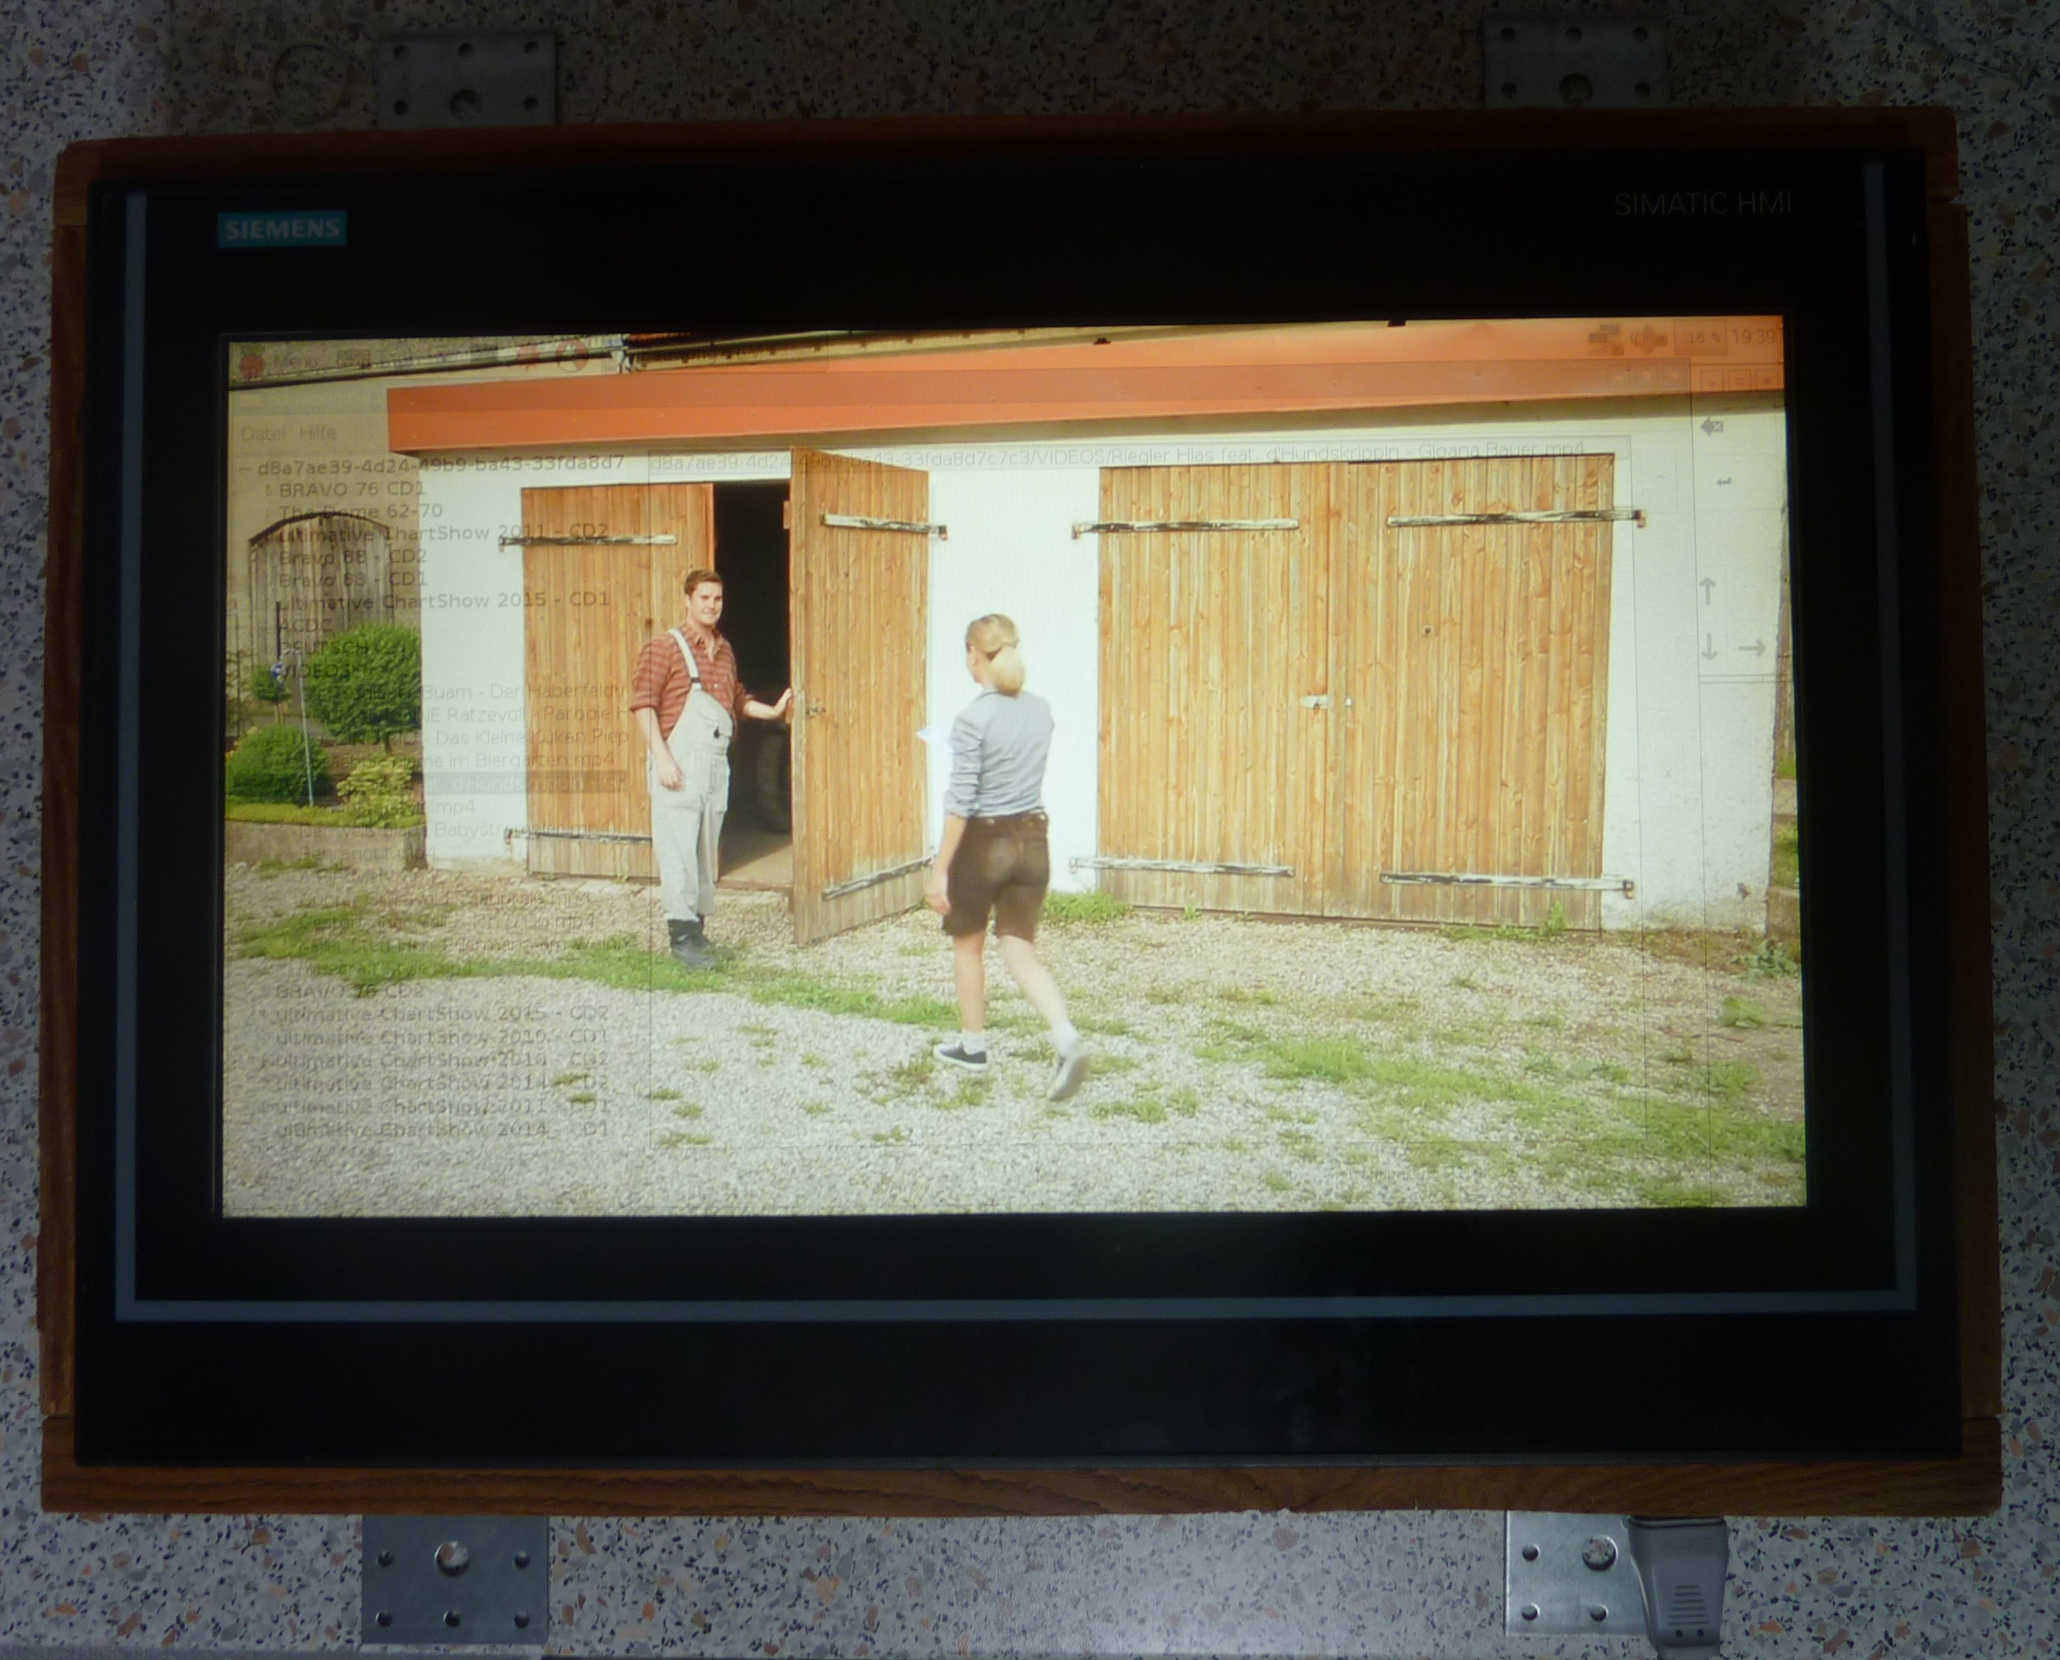
\includegraphics[width=12cm]{Titelbild.jpg}
\end{figure}

%%------------------------------------------------------------------------------
%%   CE und Firmenadresse
%%------------------------------------------------------------------------------
\begin{tabular}{p{6cm} p{6cm} p{2cm}}\\
\hline
% --- Zeile mit dem offiziellen Logo der Free Software Foundation:
%\parbox[c]{1em}{\includegraphics[width=1in]{CE.png}} & PAK GmbH, Pf<E4>lzerstra<DF>e 1\newline D-83109 Gro<DF>karolinenfeld   & Datum:\newline 07.11.2014\\
\parbox[c]{1em}{
\includegraphics[width=1in]{GPLv3_Logo.png}} & GNU General Public License v3 \newline \copyright\ \jahr\ \autor & Datum:\newline 01.07.2016\\ %{\includegraphics[width=1in]{Official_gnu.png}}\\
%\parbox[c]{1em}{\includegraphics{Official_gnu.png}} {\Bezeichnung} -- {\BezeichnungLang} {\Version}\newline (C) 2016 schlizbaeda, GNU GPL v3 & Datum:\newline 20.02.2016
% --- Zeile ohne CE-Zeichen:
%\parbox[c]{0em} \ PAK GmbH & Pf�lzerstra�e 1\newline D-83109 Gro�karolinenfeld   & Datum:\newline 07.11.2014\\

\hline
\end{tabular}
\\[4ex]

%\copyright\ \jahr\\

%\includegraphics[width=1in]{EQM_Zert.png}
\end{center}

\textbf{}\\
\textbf{}\\
Die Abbildung auf dem Display stammt aus dem Video zu folgendem Musikst�ck:\\
\texttt{\textbf{Riegler Hias feat. d' Hundskrippln} \textit{Gloana Bauer}} bei 2:42\\
\url{http://www.hundskrippln.de/#filme} %-- 2:42


\end{titlepage}




\include{Layout/Abstract}
\cfoot{- \pagemark ~-}

\tableofcontents          % Inhaltsverzeichnis
\listoffigures            % Abbildungsverzeichnis
\listoftables             % Tabellenverzeichnis
\renewcommand{\lstlistlistingname}{Verzeichnis der Listings}
%\lstlistoflistings        % Listings-Verzeichnis

% Abk�rzungsverzeichnis --------------------------------------------------------
%% Abk�rzungsverzeichnis:
%% --------------------------------------------------------------------
%\nomenclature{API}{Application Programming Interface}
%\nomenclature{ARIS}{Architektur integrierter Informationssysteme}
%\nomenclature{BPR}{Business Process Reengineering}
%\nomenclature{eEPK}{erweiterte Ereignisgesteuerte Prozesskette}
%\nomenclature{EPK}{Ereignisgesteuerte Prozesskette}
%\nomenclature{JMS}{Java Message Service}
%\nomenclature{SDK}{Software Development Kit}
%\nomenclature{URI}{Uniform Resource Identifier}
%\nomenclature{URL}{Uniform Resource Locator}
%\nomenclature{URN}{Uniform Resource Name}
%\nomenclature{W3C}{World Wide Web Consortium}
%\nomenclature{XML}{Extensible Markup Language}
%\nomenclature{XPath}{XML Path Language}
%\nomenclature{XSL}{Extensible Stylesheet Language}
%\nomenclature{XSLT}{XSL Transformations}

%\begin{itemize}
%\item	gLOSSAR1
%\item	Glossar2
%\end{itemize}

% f�r korrekte �berschrift in der Kopfzeile
\clearpage\markboth{\nomname}{\nomname} 
\printnomenclature
\label{sec:Glossar}


% arabische Seitenzahlen im Hauptteil ------------------------------------------
\clearpage
\pagenumbering{arabic}


% ##############################################################################
% ----------   Die Inhaltskapitel werden inkludiert    -------------------------
% ##############################################################################
\chapter{Einf�hrung}
\label{cha:Einfuehrung}
Ausgabest�nde dieser Dokumentation:
\begin{acronym}[]
	\acro{Version 1}{20.02.2016: Erstversion}
	\acro{Version 2}{01.07.2016: zus�tzliche Hinweise zur Software-Installation}
\end{acronym}

\section{Kurzbeschreibung}
\subsection{Software}
\label{sec:Einfuehrung_Software}
"`\Bezeichnung"' \bzw "`\BezeichnungLang"' ist ein in \textbf{Python3}
erstellter Wrapper f�r den Mediaplayer \textbf{\filenam{omxplayer.bin}}, welcher
optimal auf die Hardware des \RPi\ zugeschnitten ist. Neben der Steuerung von
\textbf{\filenam{omxplayer.bin}} �ber Kommandozeilenparameter oder die Tastatur
("`hot keys"') ist auch eine Kommunikation mittels \textbf{D-Bus} m�glich.\\
Die urspr�ngliche Absicht war, eine Software zu erstellen, mit der eine einfache
und intuitive Handhabung einer Musiksammlung m�glich ist. Dabei sollte sich die
Bedienung an einem klassischen CD-Spieler orientieren. Unter Linux und somit
auch auf dem \RPi\ gibt es das hervorragende Softwarepaket \textbf{MPD} ("`Music
Player Daemon"'), das \ua �ber ALSA alle auf dem Computer installierten
Soundkarten unterst�tzt und zahlreiche Client-Anwendungen (MPC) zur Verf�gung
stellt. Sein einziger Nachteil liegt in der Verwaltung der Musikdateien �ber
eine Datenbank und den damit verbundenen umst�ndlichen und aufw�ndigen
Aktualisierungsarbeiten bei neuen Musikdateien, die dem einfachen
CD-Spieler-Prinzip entgegenstehen. \textit{Gerne lasse ich mich hier vom
Gegenteil �berzeugen, falls es f�r den \RPi\ taugliche MPCs geben sollte
\smiley{wink}} (\url{mailto:schlizbaeda@gmx.de}).\\
Die Software \textbf{\Bezeichnung} in Version \Version\ besteht aus einer
grafisch einfach gehaltenen, mit dem Python-Modul \textbf{tkinter} erstellten
Benutzeroberfl�che (GUI) �hnlich einem Dateimanager: Im linken Teil befindet
sich ein sogenanntes Treeview-Steuerelement, in dem die hierarchische
Ordnerstruktur von Laufwerken angezeigt wird, die unter \filenam{/media}
gemountet sind. Am \RPi\ neu angeschlossene USB-Laufwerke werden automatisch
erkannt und entsprechend in die Ordnerstruktur eingebunden. Musikdateien k�nnen
durch eine Doppelklick in die Playlist eingetragen werden.\\
Der rechte Teil besteht aus der Playlist und Steuerelementen zum Entfernen und
Verschieben der Musiktitel innerhalb der Playlist. Im unteren Teil befinden sich
die Steuerelemente zum Abspielen der Musiktitel, wie man sie vom CD-Spieler
kennt, au�erdem ist noch ein Eingabefeld f�r die Titelsuche enthalten.

\subsection{Hardware}
\label{sec:Einfuehrung_Hardware}
Grunds�tzlich ist f�r den Betrieb von \textbf{\Bezeichnung} nur ein \RPi\
erforderlich, an den ein HDMI-Bildschirm mit Lautsprechern angeschlossen wird.
F�r die Bedienung ben�tigt man ferner ein Touchpanel oder Tastatur und Maus.\\
Der erste konkrete Anwendungsfall f�r \textbf{\Bezeichnung} war jedoch ein
Musikspieler auf dem Faschingswagen 2016 mit dem Thema "`500 Jahre
Reinheitsgebot"' von \Verein{\bauwong}, einer losen Gruppe von Freunden in
Gro�karolinenfeld. In der weisen Voraussicht, dass es auf dem Wagen w�hrend der
Teilnahme an den Faschingsumz�gen mitunter auch etwas grob zugehen k�nnte,
beschloss ich, anstatt meines Laptops einen Aufbau mit robusteren und
gleichzeitig kosteng�nstigeren Komponenten umzusetzen, die den mechanischen
Anforderungen standhalten sollten:\\
Ein \textbf{SIMATIC Industrial Flat Panel} (19 Zoll) aus dem Hause Siemens --
nicht wirklich billig, aber dank Vitamin B bin ich daran kostenlos herangekommen
\smiley{smile.png}: Widerstandsf�hig genug, um den Anforderungen im rauhen
Industrieeinsatz zu gen�gen, sollte es auch den Einsatz auf dem Faschingswagen
aushalten.\\
Auf dem r�ckseitigen Deckel des Panels wurden ein \textbf{\RPi\ Modell B+} und
ein \textbf{\Ligawo} montiert. Letzerer ist notwendig, um aus dem HDMI-Anschluss
ein analoges Audiosignal abzugreifen. Der analoge Audioausgang des \RPi\ ist
n�mlich echt besch...eiden \smiley{nosmile}. Das Ligawoteil ist mal Chinaware,
die wirklich zu gebrauchen ist: Das erzeugte Audiosignal zeigt keinerlei
Qualit�tseinbu�en. Selbst bei gr��erer Lautst�rke an relativ guten Verst�rkern
und Lautsprechern, wo schlechte Tonqualit�t schnell auff�llt, konnte ich als
relativ anspruchsvoller HiFi-Fan keine Abstriche erkennen. \smiley{smile}\\
Das Ganze wurde in ein zugegebenerma�en rustikales Holzgeh�use eingebaut (siehe
Bilder), Netzteile (24V und 5V) rein, 230V-, USB- und Ethernet-Buchsen sowie
drei Schalter ins Holzgeh�use gebaut, das Zeug noch intern verkabelt und fertig.

 
\newpage
\section{Rechtliche Hinweise zu Lizenz, Gew�hrleistung und Links}
\subsection{Software unter GPL v3 }
Die Software \textbf{\Bezeichnung} wird unter der Lizenz GPL v3 der \Verein{Free
Software Foundation} ver�ffentlicht. Die Software darf frei kopiert und  privat
oder kommerziell gem�� den Lizenzvorgaben verwendet werden. Bitte lesen Sie die
GPL v3, die sich im Programmpaket in der Datei \filenam{bauwong.lic} befindet
oder laden Sie den Originaltext aus dem Internet von
\url{https://www.gnu.org/licenses/gpl-3.0} herunter.

\autor\ als Urheber und Copyrightinhaber stellt die Software "`so wie sie ist"'
ohne Garantie und ohne Zusicherung einer bestimmten Funktionalit�t zum Download
bereit. Es steht Ihnen als Anwender frei, die Software zu benutzen oder es eben
nicht zu tun. Entscheiden Sie sich f�r die Benutzung, so tun Sie dies auf
eigenes Risiko und auf eigene Verantwortung. Der Autor �bernimmt keine Garantie
f�r die Software und deren Funktion und haftet auch nicht f�r Sch�den, die aus
der Installation und Verwendung der Software entstehen.

\subsection{Dokumentation unter FDL v1.3}
Diese Dokumentation wurde mit dem Textsatzsystem \LaTeX\ erstellt.\\
Sie darf gem�� der Bestimmungen aus der Lizenz FDL v1.3 (oder nachfolgend)
kopiert, verteilt und/oder ge�ndert werden. Details siehe 
\url{http://www.gnu.org/licenses/fdl.html}

\subsection{Externe Internet-Links}
\textbf{Einfach weil's sein muss:}\\
In diesem Dokument befinden sich Links zu verschiedenen externen Seiten im
Internet. Den Inhalt mache ich mir nicht zu eigen, da ich auf die Gestaltung
dieser Seiten keinerlei Einfluss habe. Zum Zeitpunkt der Verlinkung enthielt
keine Seite illegale Inhalte. Dies kann ich aber nur in gr��eren Abst�nden
kontrollieren. Sollten Sie an einem Link etwas auszusetzen haben, so senden Sie
bitte eine e-mail an \url{mailto:schlizbaeda@gmx.de}. 


\section{Konventionen dieser Dokumentation}

%----------------------------------------------------------------------
%----HINWEISBOX---- (keinRahmen und Gl�hbirne als Symbol)
%----------------------------------------------------------------------
%\begin{bclogo}[logo = \bclampe, noborder = true]{Hinweis}
%Optional befinden sich die Ausschnitte f�r zwei weitere USB Schnittstellen, zwei weitere LAN Buchsen sowie eine weitere 37-polige Sub-D Schnittstelle
%am �bergabefeld der Zelle.
%\end{bclogo}

Folgende gestalterische Konventionen werden f�r die Dokumentation festgelegt:

\begin{table}[!h]
\centering
\renewcommand{\arraystretch}{2}
\begin{tabular}{|p{4cm}|p{10cm}|}
\hline
\parbox[c]{1em}{\begin{bclogo}[logo = \bclampe, noborder = true]{Hinweis}
Text
\end{bclogo}}
	& Ein Hinweis enth�lt zus�tzliche Information bzw. relevante Erl�uterung zu einer bestimmten Funktionalit�t\\
\hline
\parbox[c]{4cm}{\begin{bclogo}[arrondi = 0.2, logo = \bcinfo, ombre = true, epOmbre = 0.25, couleurOmbre = black !30,blur]{Achtung}
Text
\end{bclogo}}	& Ein Warnhinweis, dessen Nichtbeachtung zu Ger�tesch�den f�hren kann\\
\hline
\button{Schaltfl�che} & Kennzeichnung von Schaltfl�chen der Software \textbf{\Bezeichnung}\\
\hline
\menuitem{Men�punkt} & Kennzeichnung von Men�punkten der Software \textbf{\Bezeichnung}\\
\hline
\prompt{Meldung} & Kennzeichnung von Meldungen der Software \textbf{\Bezeichnung}\\
\hline
\end{tabular}
\vspace{0.5cm}
\caption{Konventionen der Dokumentation}
\end{table}


\section{Abk�rzungsverzeichnis}
Folgende Abk�rzungen werden in dieser Dokumentation verwendet:
\begin{acronym}[\Bezeichnung]
	\acro{ALSA}{\textbf{A}dvanced \textbf{L}inux \textbf{S}ound \textbf{A}rchitecture}
	\acro{D-Bus}{\textbf{D}esktop-\textbf{Bus}}
	\acro{DVI}{\textbf{D}igital \textbf{V}isual \textbf{I}nterface}
	\acro{GUI}{\textbf{G}raphical \textbf{U}ser \textbf{I}nterface}
	\acro{HDMI}{\textbf{H}igh \textbf{D}efinition \textbf{M}ultimedia \textbf{I}nterface}
	\acro{MPC}{\textbf{M}usic \textbf{P}layer \textbf{C}lient}
	\acro{MPD}{\textbf{M}usic \textbf{P}layer \textbf{D}aemon}
	\acro{USV}{\textbf{U}nterbrechnungsfreie \textbf{S}trom\textbf{v}ersorgung}
\end{acronym}


\chapter{Hardware}
\label{cha:Hardware}


\section{Hinweise zum Nachbau der Hardware}
Dieses Kapitel der Dokumentation beschreibt die f�r meine Anwendung von
\Bezeichnung\ aufgebaute Hardware, ein Touchpanel mit einem \RPi\ Modell B+ und
allen notwendigen Komponenten, die zur Verwendung als Audioquelle in der
Musikanlage unseres Faschingswagens notwendig waren.

\begin{figure}[!h]
\centering

\includegraphics[width=4cm]{elektrischeSpannung.png}
\caption{Gef�hrliche elektrische Spannung}
%\label{fig:elektrSpann}
\end{figure}

F�r den beschriebenen Aufbau wurde eine Spannungsversorgung �ber 12V-Bleiakkus
verwendet (gro�e LKW-Batterien). �ber einen 12V/230V-Spannungswandler wird die
Betriebsspannung f�r die im RPi-Touchpanel verbauten Netzteile erzeugt.

\begin{bclogo}[arrondi = 0.2, logo = \bcinfo, ombre = true, epOmbre = 0.25, couleurOmbre = black !30,blur]{Vorsicht!}
Ich appelliere an die Vernunft der Leserschaft, den Nachbau nur vorzunehmen,
wenn man sich folgender Gefahren bewusst ist und das fachliche Wissen und
handwerkliche K�nnen besitzt, sie zu vermeiden:
\begin{itemize}
\item ausgehende Gefahr von einer 230V-Wechselspannung (gef�hrlicher Stromschlag)
\item ausgehende Gefahr von hohen Str�men aus Autobatterien (Kurzschlussfall!)
\end{itemize}
\end{bclogo}

\textbf{Lizenz:}\\
Der hier beschiebene elektrische Aufbau erreicht nicht die sch�pferische Tiefe,
um �ber eine Lizenz gesch�tzt werden zu m�ssen. Vielmehr beruht er auf den
allgemein bekannten Fakten f�r die Inbetriebnahme eines \RPi\ sowie auf den
Bedienungsanleitungen der verwendeten Einzelkomponenten.\\


\section{Blockschaltbild}
Eine kurze funktionale Beschreibung des Aufbaus ist bereits in Kapitel
\ref{sec:Einfuehrung_Hardware} erfolgt. Aufgrund einer �u�erst kurzfristigen
�nderung der Rahmenbedingungen musste die Stromversorgung neu gestaltet werden.
Daher wurde (gezwungenerma�en aus Zeit- und Materialmangel) auf eine saubere
Netzabschaltung verzichtet. Die Spannungsversorgung der Einzelkomponenten
(Siemens IFP, \Ligawo, \RPi) kann jedoch �ber einzelne Schalter getrennt
zugeschaltet werden, um die Komponenten in einer definierten Reihenfolge in
Betrieb zu nehmen. Siehe dazu auch Kapitel \ref{subsec:PowerSequencer},
Abschnitt "`Power Sequencer"'\\
F�r einen vollst�ndigen �berblick hier ein Blockschaltbild:
\begin{figure}[!h]
\centering
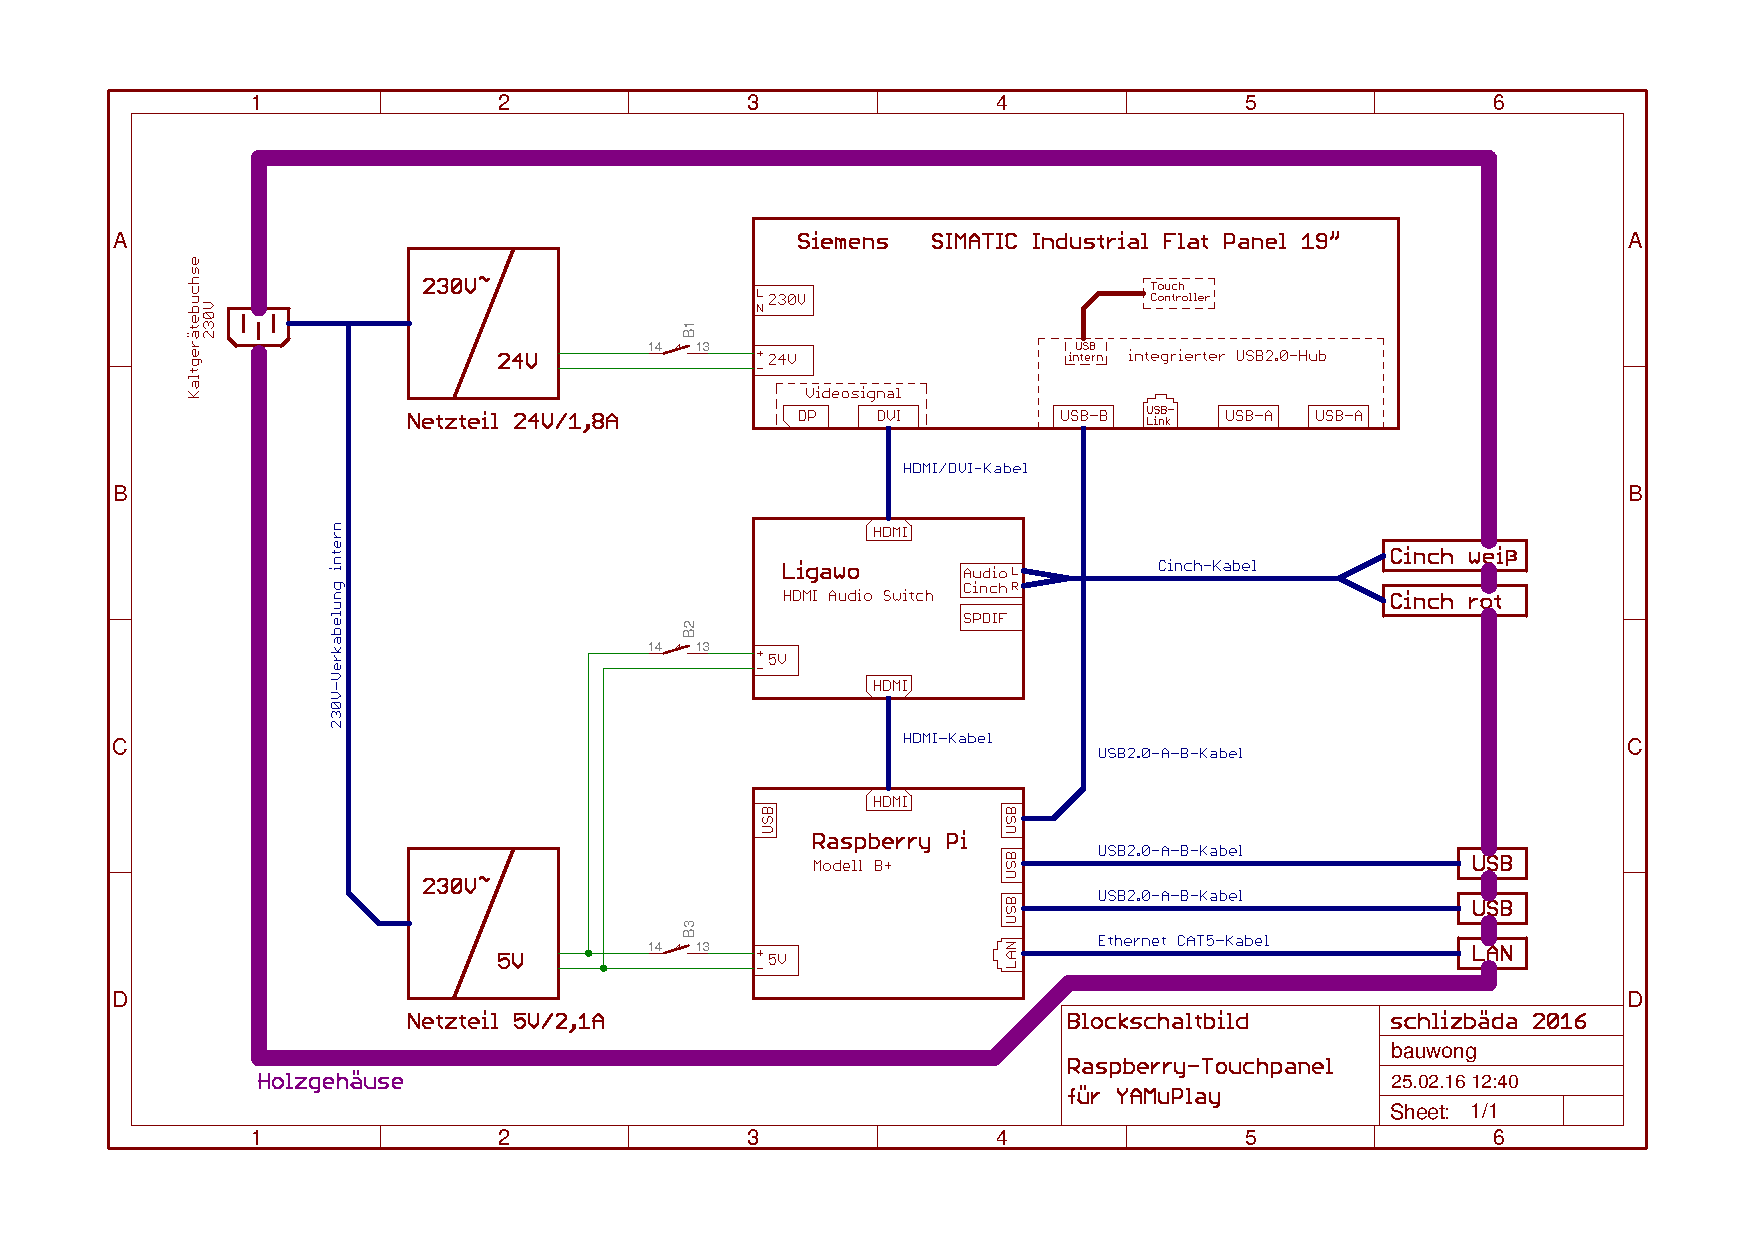
\includegraphics[width=\textwidth]{Blockschaltbild.pdf}
\caption{Blockschaltbild}
\label{fig:Blockschaltbild}
\end{figure}


\newpage
\section{St�ckliste}
Folgende Komponenten wurden f�r den elektrischen Aufbau verwendet. Das Material
f�r den Holzrahmen (Holz, Schrauben, Montagewinkel) ist in der St�ckliste nicht
aufgef�hrt.

\begin{table}[!h]
\centering
\renewcommand{\arraystretch}{1.5}
\begin{tabular}{|l|l|l|p{0.45\textwidth}|}
\toprule[2pt]
\textbf{Anz.} & \textbf{Lieferant} & \textbf{Bestellnummer} & \textbf{Artikel}\\
\midrule[2pt]
1 & Vitamin B \smiley{wink} & --- & Siemens IFP 19" MultiTouch\\
\hline
1 & Vitamin B \smiley{wink} & --- & Deutronic Einbaunetzteil 24V / 1.8A\\
\hline
1 & amazon & Ligawo 6518725 & Ligawo 6518725 HDMI Extractor\\
\hline
1 & www.raspiprojekt.de & 35001 & \RPi\ Modell B+\\
\hline
1 & reichelt & GOO 44009 & 5V-USB-Netzteil, 2A (USB-Ladeadapter)\\
\hline
1 & reichelt & KES 1 & Kaltger�teeinbaustecker, waagerecht befestigt\\
\hline
3 & reichelt & WIPPE 1801.1146 & Marquardt Wippschalter 1-pol\\
\hline
1 & reichelt & NEUTRIK NF2DB-2 & Cincheinbaubuchse, Farbkennring rot\\
\hline
1 & reichelt & NEUTRIK NF2DB-9 & Cincheinbaubuchse, Farbkennring wei�\\
\hline
1 & reichelt & NEUTRIK NE-8FDP & Flanschbuchse RJ45 auf RJ45\\
\hline
2 & reichelt & NEUTRIK NAUSB-WB & USB-Einbaudurchgangsbuchse, innen USB-B, au�en USB-A\\
\hline
1 & reichelt & AK HDMI-DVI 1,0 & HDMI-Stecker auf DVI-D Stecker 1,0m\\
\hline
1 & reichelt & AK HDMI 0,50G ET & HDMI Kabel Stecker/Stecker 0,5m\\
\hline
1 & reichelt & AVK 128 & 2x Cinchstecker auf 2x Cinchstecker 1,5m \\
\hline
3 & reichelt & AK 672/HSF-0,5 & USB2.0-Kabel, A-Stecker auf B-Stecker 0,5m\\
\hline
1 & reichelt & PATCH-C7 05 MA & 0,5m Cat.7 PiMF-Patchkabel, magenta, RJ45\\
%\hline
\bottomrule[2pt]
\end{tabular}
\vspace{0.5cm}
\caption{St�ckliste}
\label{tab:Stueckliste}
\end{table}


\newpage
\section{Ausblick und m�gliche Verbesserungen}
Die hier beschriebene Umsetzung ist lediglich als Anregung zu verstehen: Es
wurde hier ganz bewusst auf eine massive Bauweise gesetzt und hinsichtlich der
mechanischen Beanspruchung f�r die geplante Anwendung (Faschingswagen!) auf
robuste Komponenten wie ein industrielles Touchpanel Wert gelegt. Das Innenleben
hinter dem Touchpanel im Holzrahmen konnte dann entsprechend filigraner
umgesetzt werden.\\
Je nach Verwendung und Einsatzort eignet sich allerdings jedes beliebige andere
Display mit HDMI-Anschluss mit einer Aufl�sung von mindestens 1366x768 Pixeln.
Anstelle der Touchfunktionalit�t k�nnen auch eine ganz normale Tastatur und
Maus benutzt werden.

Nachdem zun�chst geplant war, eine 230V-Stromversorgung �ber ein am Bulldog
angeschlossenes Zapfwellenaggregat herzustellen und mit gro�en Verst�rkern zu
arbeiten, musste ich dann feststellen, dass die Drehrichtung der Zapfwelle vorne
genau falsch herum war. Da das Aggregat Drehstrom erzeugt, muss auch die
Drehrichtung stimmen: Man denke an eine Drehstrom-Kreiss�ge, deren S�geblatt
sich falsch herum dreht... Saugef�hrlich! Daher schaltete bei unserem Aggregat
die Sicherungseinrichtung ab. \smiley{nosmile} Ein Anschluss des Aggregates an
der Hinterseite des Bulldogs fiel aus, da ja dort der Faschingswagen h�ngt und
das Aggregat der Deichsel im Wege ist. \smiley{nosmile}\\
Gott sei Dank haben wir das Ganze eine Woche vor dem ersten Einsatz gepr�ft und
festgestellt, dass es nicht geht. Daher wurde ein
12V/230V-Sinus-Spannungswandler mit 1500W Dauerleistung bestellt, aber leider
billigste Chinaware bei dem gro�en Online-Versand, der in Deutschland keine
Steuern bezahlt. Ausgepackt, angeschlossen, geht nicht! \smiley{nosmile} Das
Glump daraufhin sofort wieder zur�ckgeschickt.

\textbf{Also:} Umbau am Tag vor dem ersten Faschingszug auf die althergebrachte
Weise mit Autoendstufen und einem kleinen Spannungswandler mit (angeblich) 300
Watt. Deshalb auch die f�r manchen Leser wohl relativ chaotische und
undurchdachte Spannungsversorgung im RPi-Touchpanel. Anschlie�end noch drei
Endstufen mit Frequenzweiche in den Faschingswagen gespaxt, um halb sieben
abends dann eingeschaltet, ausgepegelt und eine Halbe Bier aufgemacht.
\smiley{smile}

\begin{bclogo}[logo = \bclampe, noborder = true]{Hinweis}
Wenn die folgenden Punkte umgesetzt w�rden, k�nnte der ganze Aufbau sogar noch
gut werden!
\end{bclogo}

\begin{itemize}
\item \textbf{Saubere 230V-Versorgung mit Hauptschalter}\\
selbstredend!
\label{subsec:PowerSequencer}
\item \textbf{Power Sequencer}\\
Derzeit tritt das Problem auf, dass \textit{manchmal} nach dem Start des \RPi\
kein Ton ausgegeben wird, obwohl eigentlich alle Komponenten eingeschaltet sind.
Ich vermute die Ursache im \Ligawo. Im deutschsprachigen RaspberryPi-Forum
schildert ein Anwender n�mlich ein �hnliches Problem:\\
\url{http://www.forum-raspberrypi.de/Thread-problem-mit-hdmi-audio-extractor-ligawo?highlight=Ligawo+Audio}\\
Dies kann \textit{meistens} umgangen werden, indem zuerst der HDMI-Bildschirm,
dann der \Ligawo\ und zuletzt der \RPi\ und alles im richtigen Zeitabstand
eingeschaltet wird. \textit{So ganz sicher bin ich mir da allerdings nicht, da
selbst ich schon drei aufeinanderfolgende fehlgeschlagene Boots erlebt habe.
\smiley{nosmile}}\\
M�glicherweise k�nnte diese Einschaltreihenfolge mit einem Mikrocontroller
automatisiert werden.
\item \textbf{Sauberes Herunterfahren / USV}\\
Die obige Mikrocontrollerschaltung k�nnte so erweitert werden, dass beim
Ausschalten die Stromversorgung zum \RPi\ erst dann getrennt wird, wenn dieser
vollst�ndig heruntergefahren ist. Alternativ w�re der Einbau einer USV f�r den
\RPi\ noch eine Option, siehe \url{http://www.piusv.de}
\item \textbf{\RPi\ Modell A oder Pi Zero verwenden}
Wenn das verwendete Display einen eingebauten USB-Hub hat (so wie mein
Siemens-Panel), kann auch ein \RPi-Modell mit nur einer USB-Buchse verwendet
werden. Man stellt eine USB-Verbindung vom \RPi\ zum USB-Hub des Displays her
und verbindet dessen Ausgangs-Ports mit den im Geh�use verbauten USB-Buchsen.
Da bringe ich dann endlich meinen \RPi\ Modell A+ sinnvoll unter.
\smiley{smile}
\end{itemize}


\section{Bilder vom Aufbau}
\begin{figure}[h]
\centering
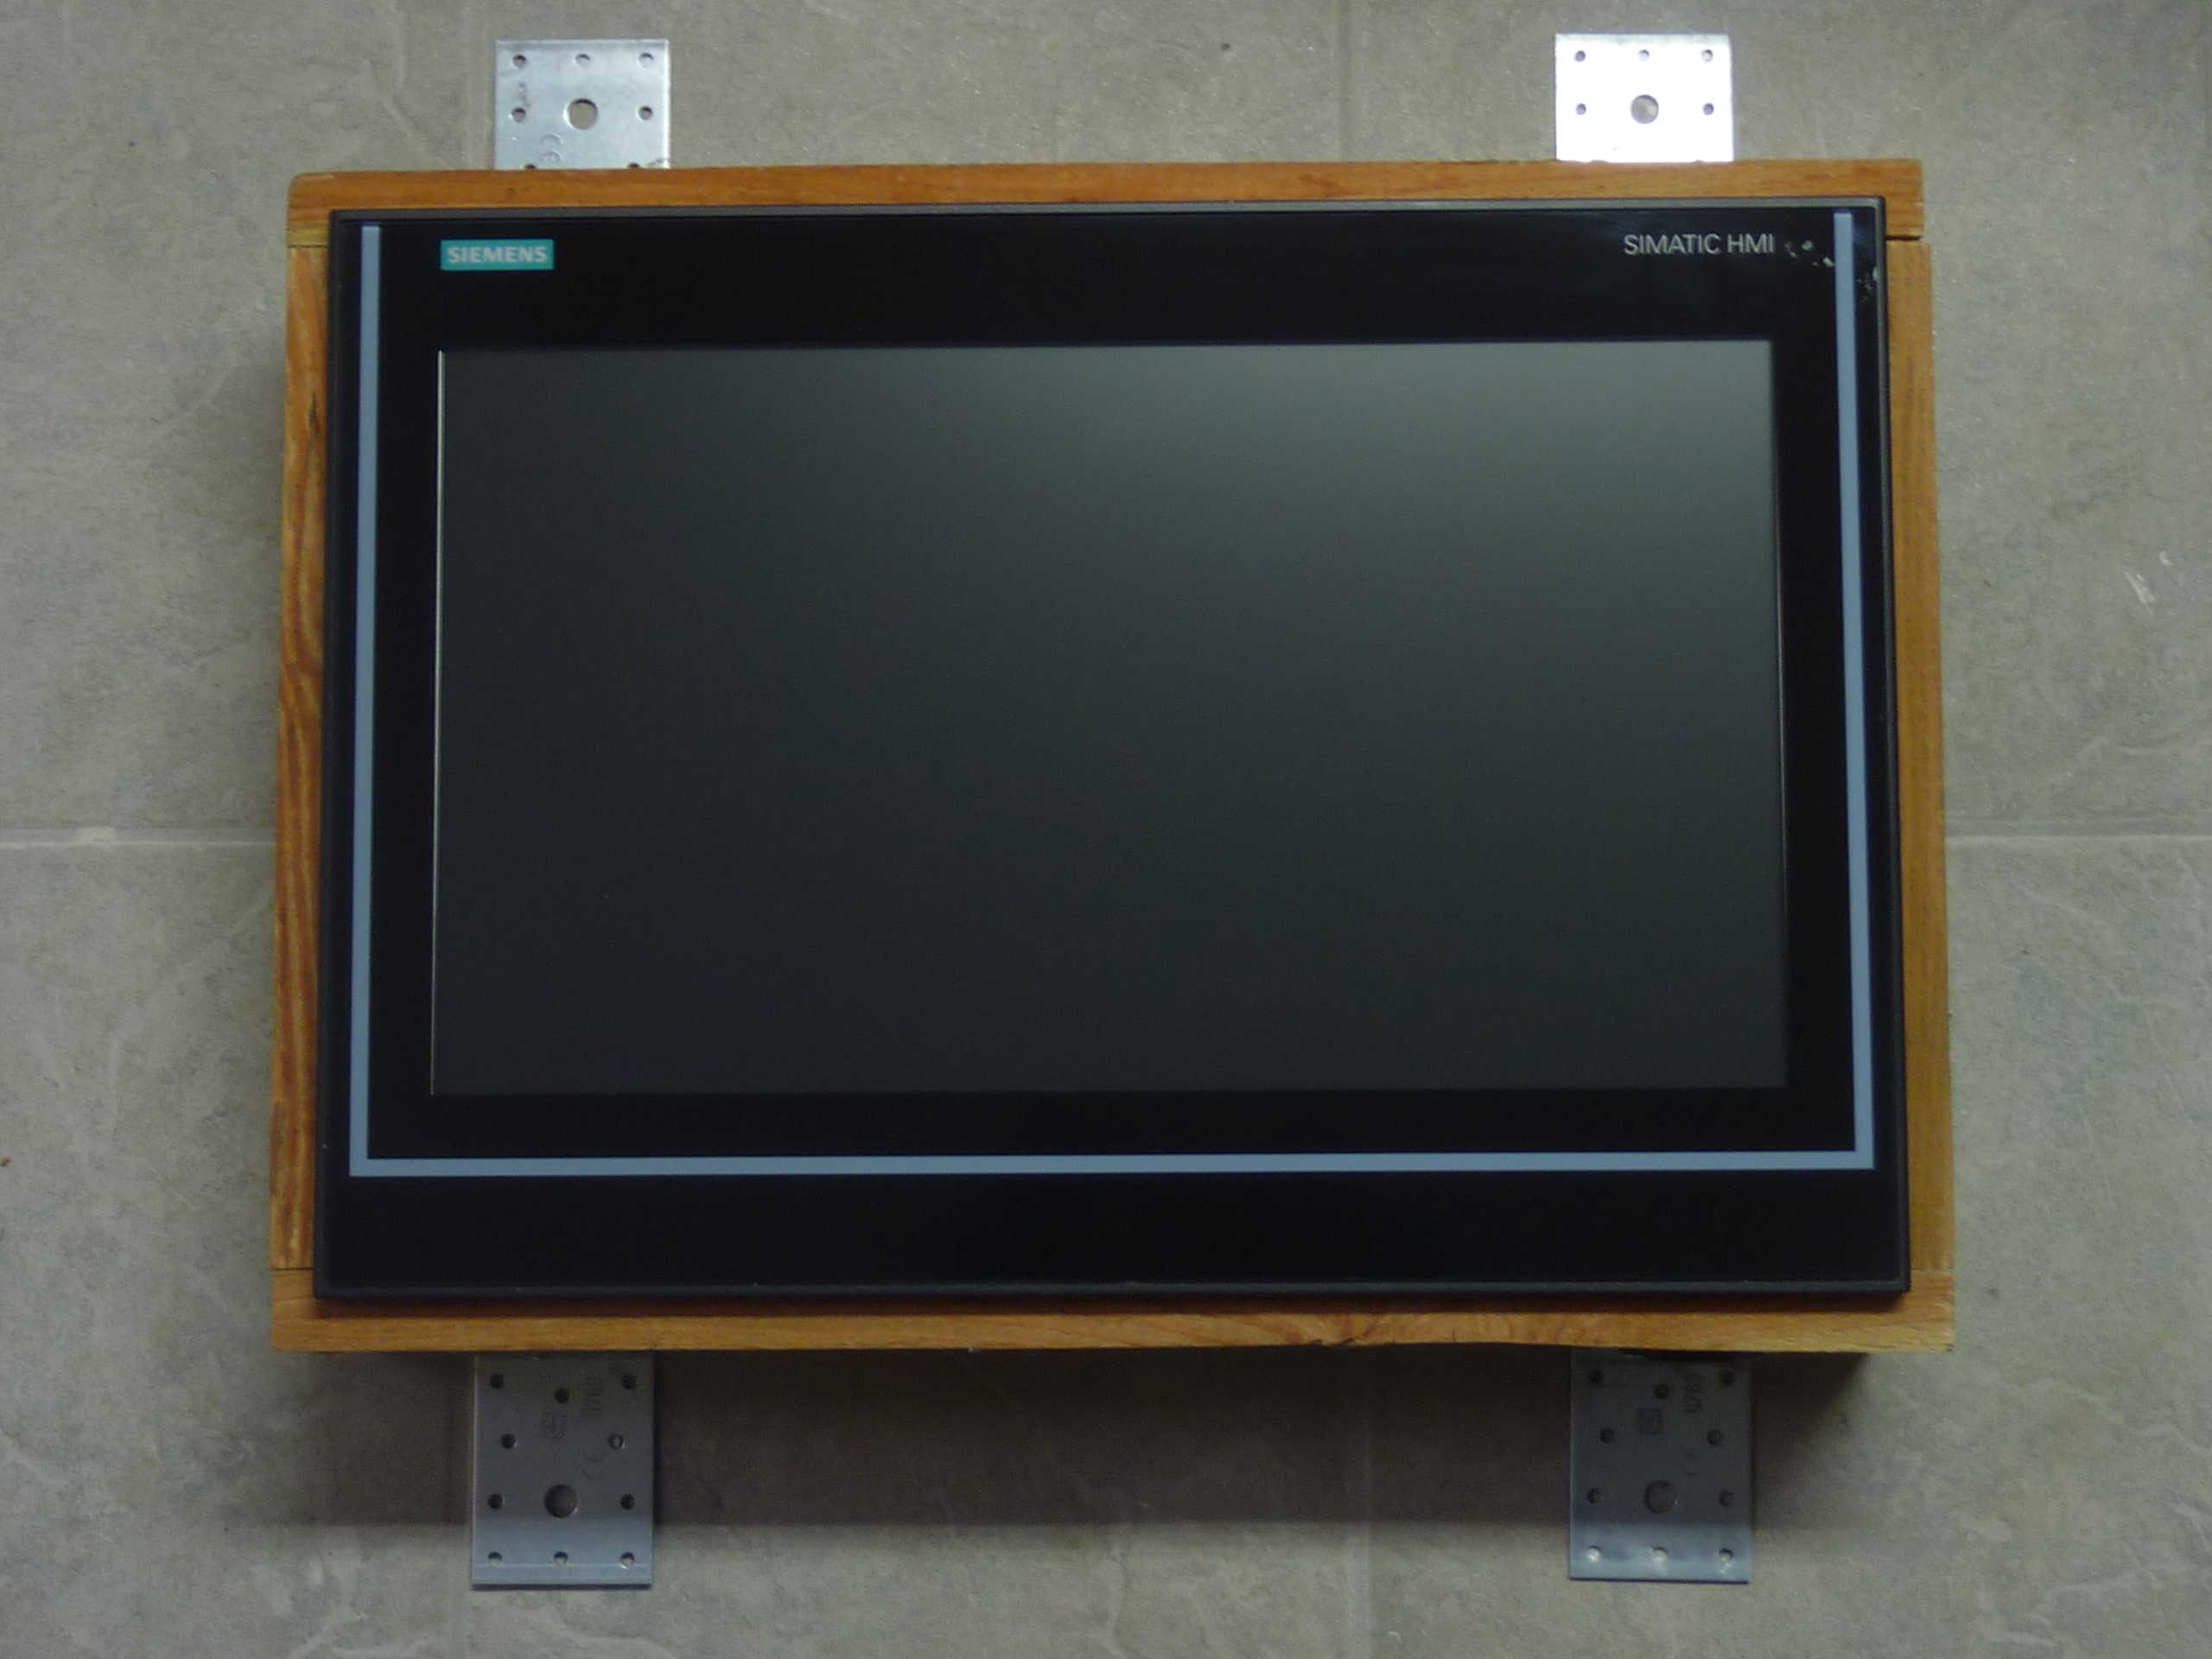
\includegraphics[width=0.67\textwidth]{RPi_YAMuPlay_Frontansicht.JPG}
\caption{Frontansicht}
\label{fig:Frontansicht}
\end{figure}

\begin{figure}[h]
\centering
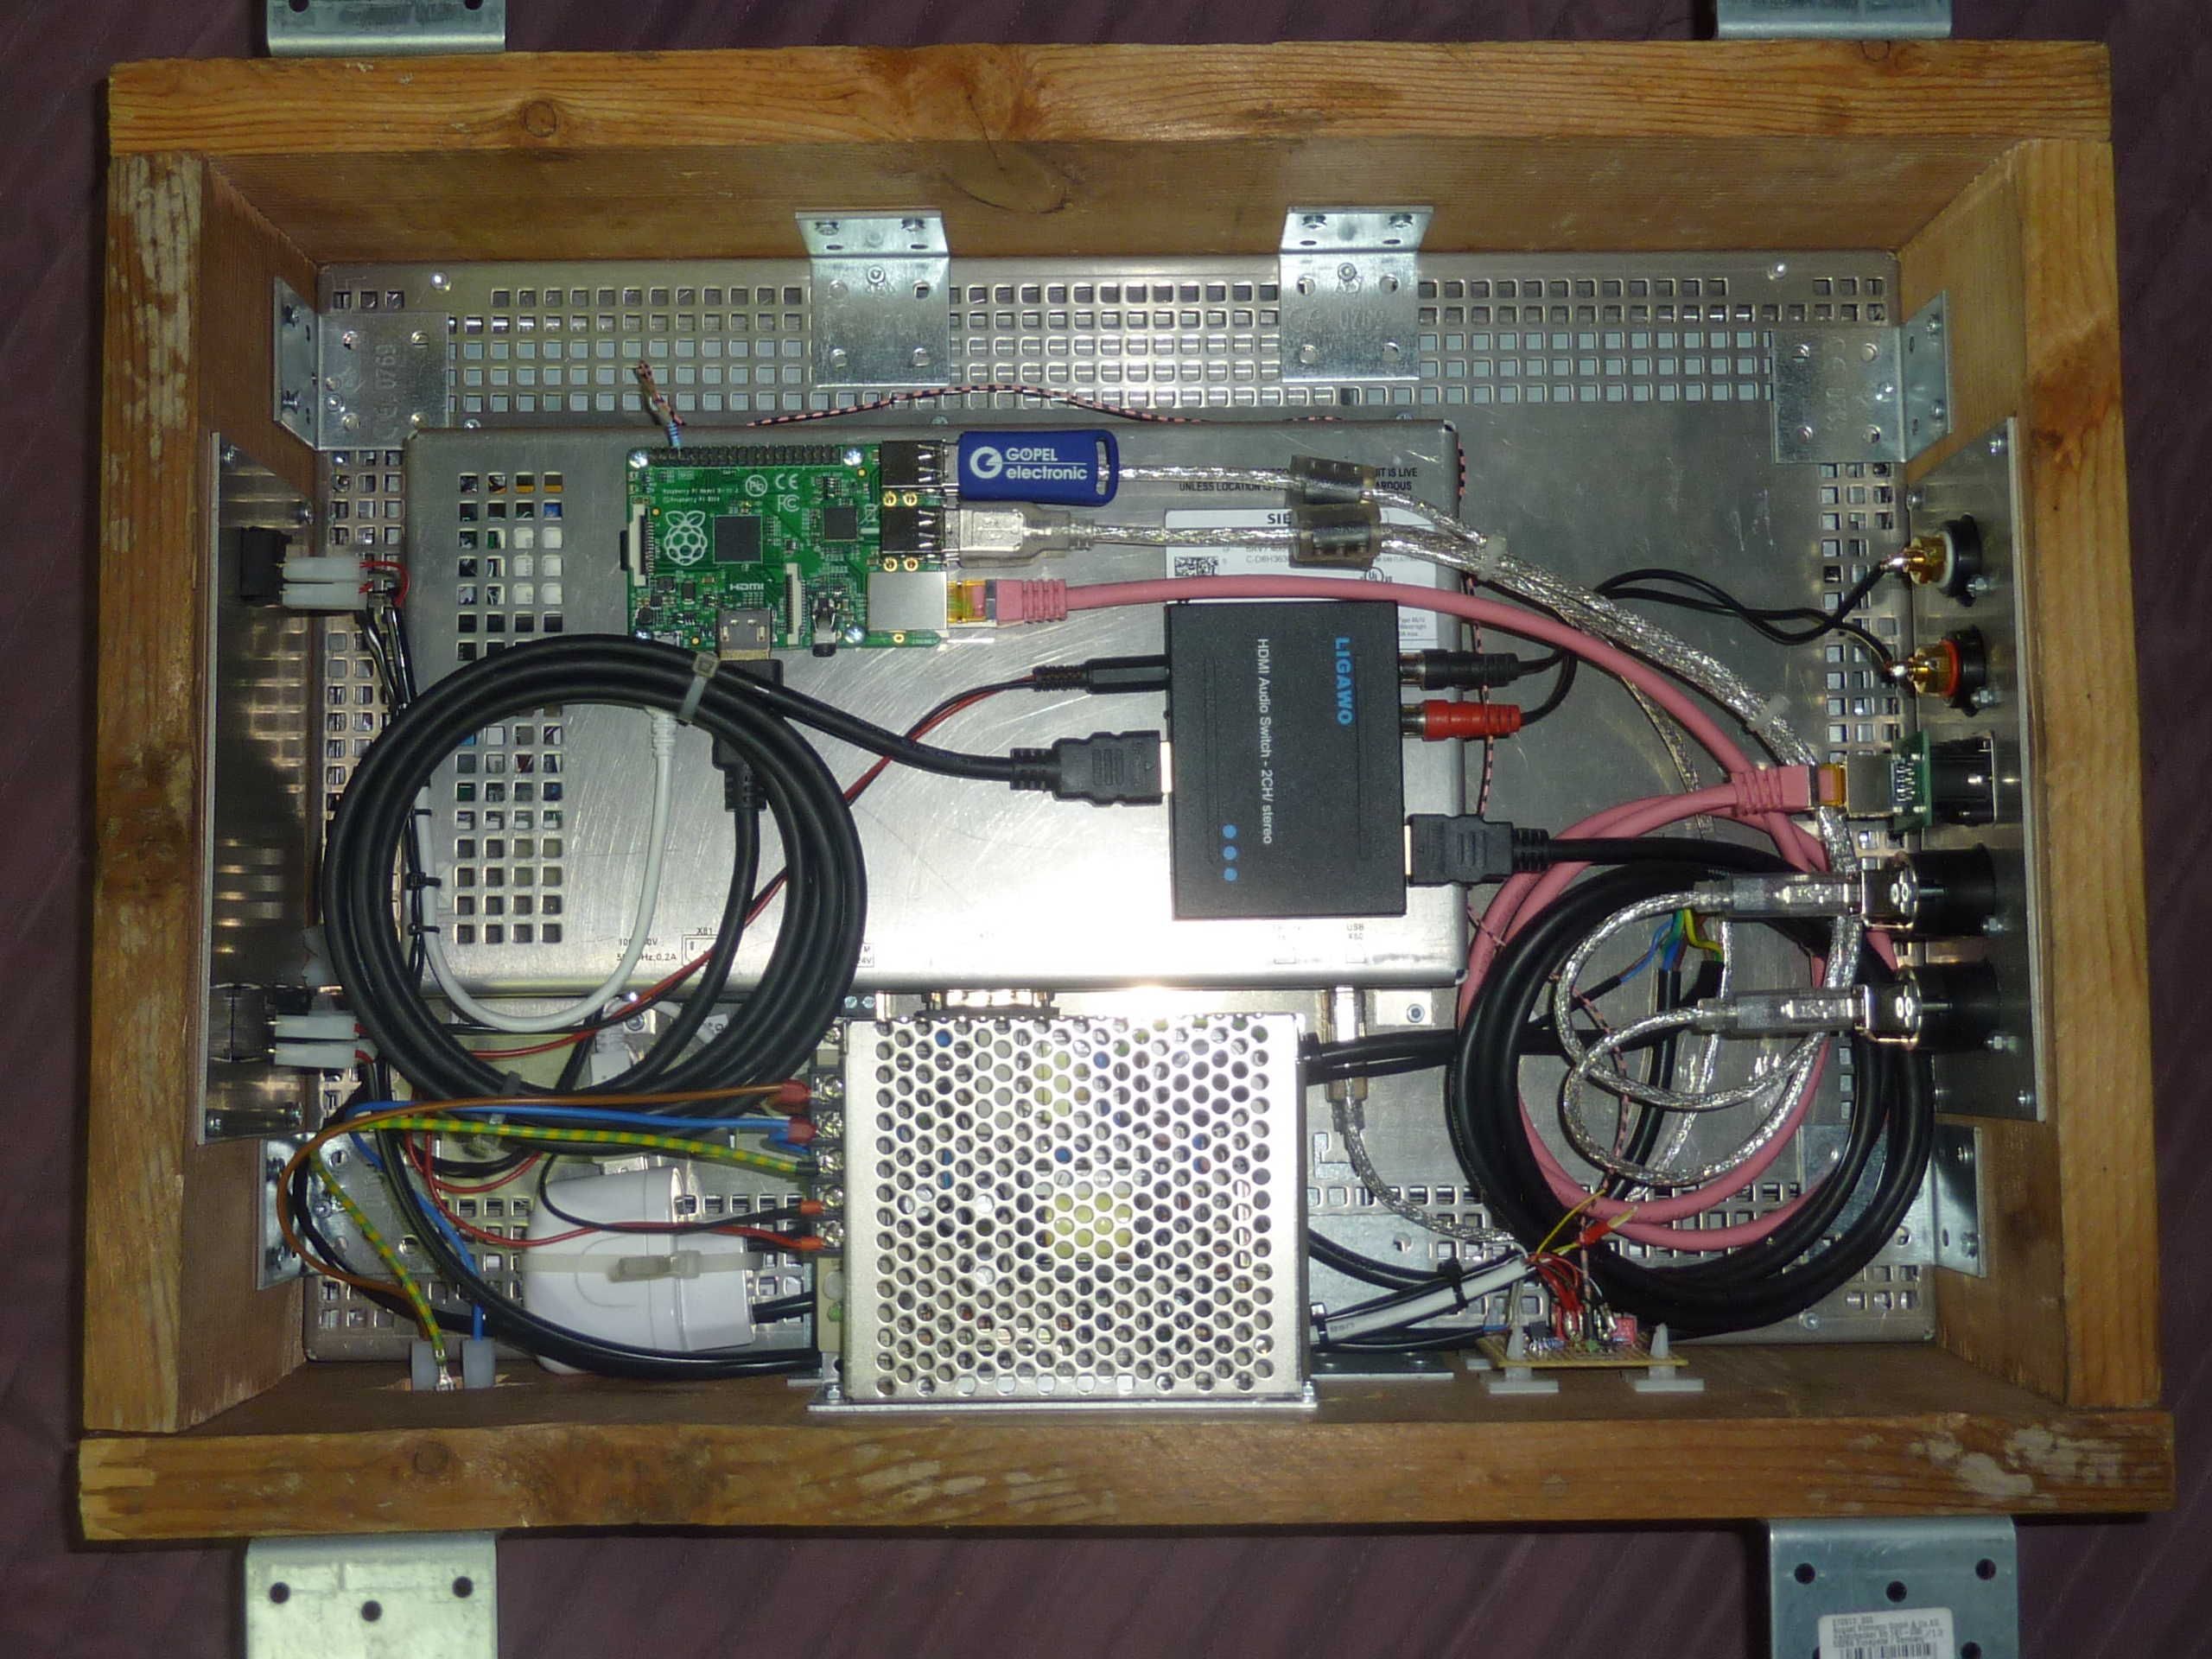
\includegraphics[width=0.8\textwidth]{RPi_YAMuPlay_Innenansicht_mit_DVI-Kabel.JPG}
\caption{Innenansicht}
\label{fig:Innenansicht}
\end{figure}

\begin{figure}[h]
\centering
\includegraphics[width=0.8\textwidth]{RPi_YAMuPlay_Innenansicht_RPi+Ligawo.JPG}
\caption{Detailansicht \RPi\ und \Ligawo}
\label{fig:Detailansicht}
\end{figure}

\begin{figure}[h]
\centering
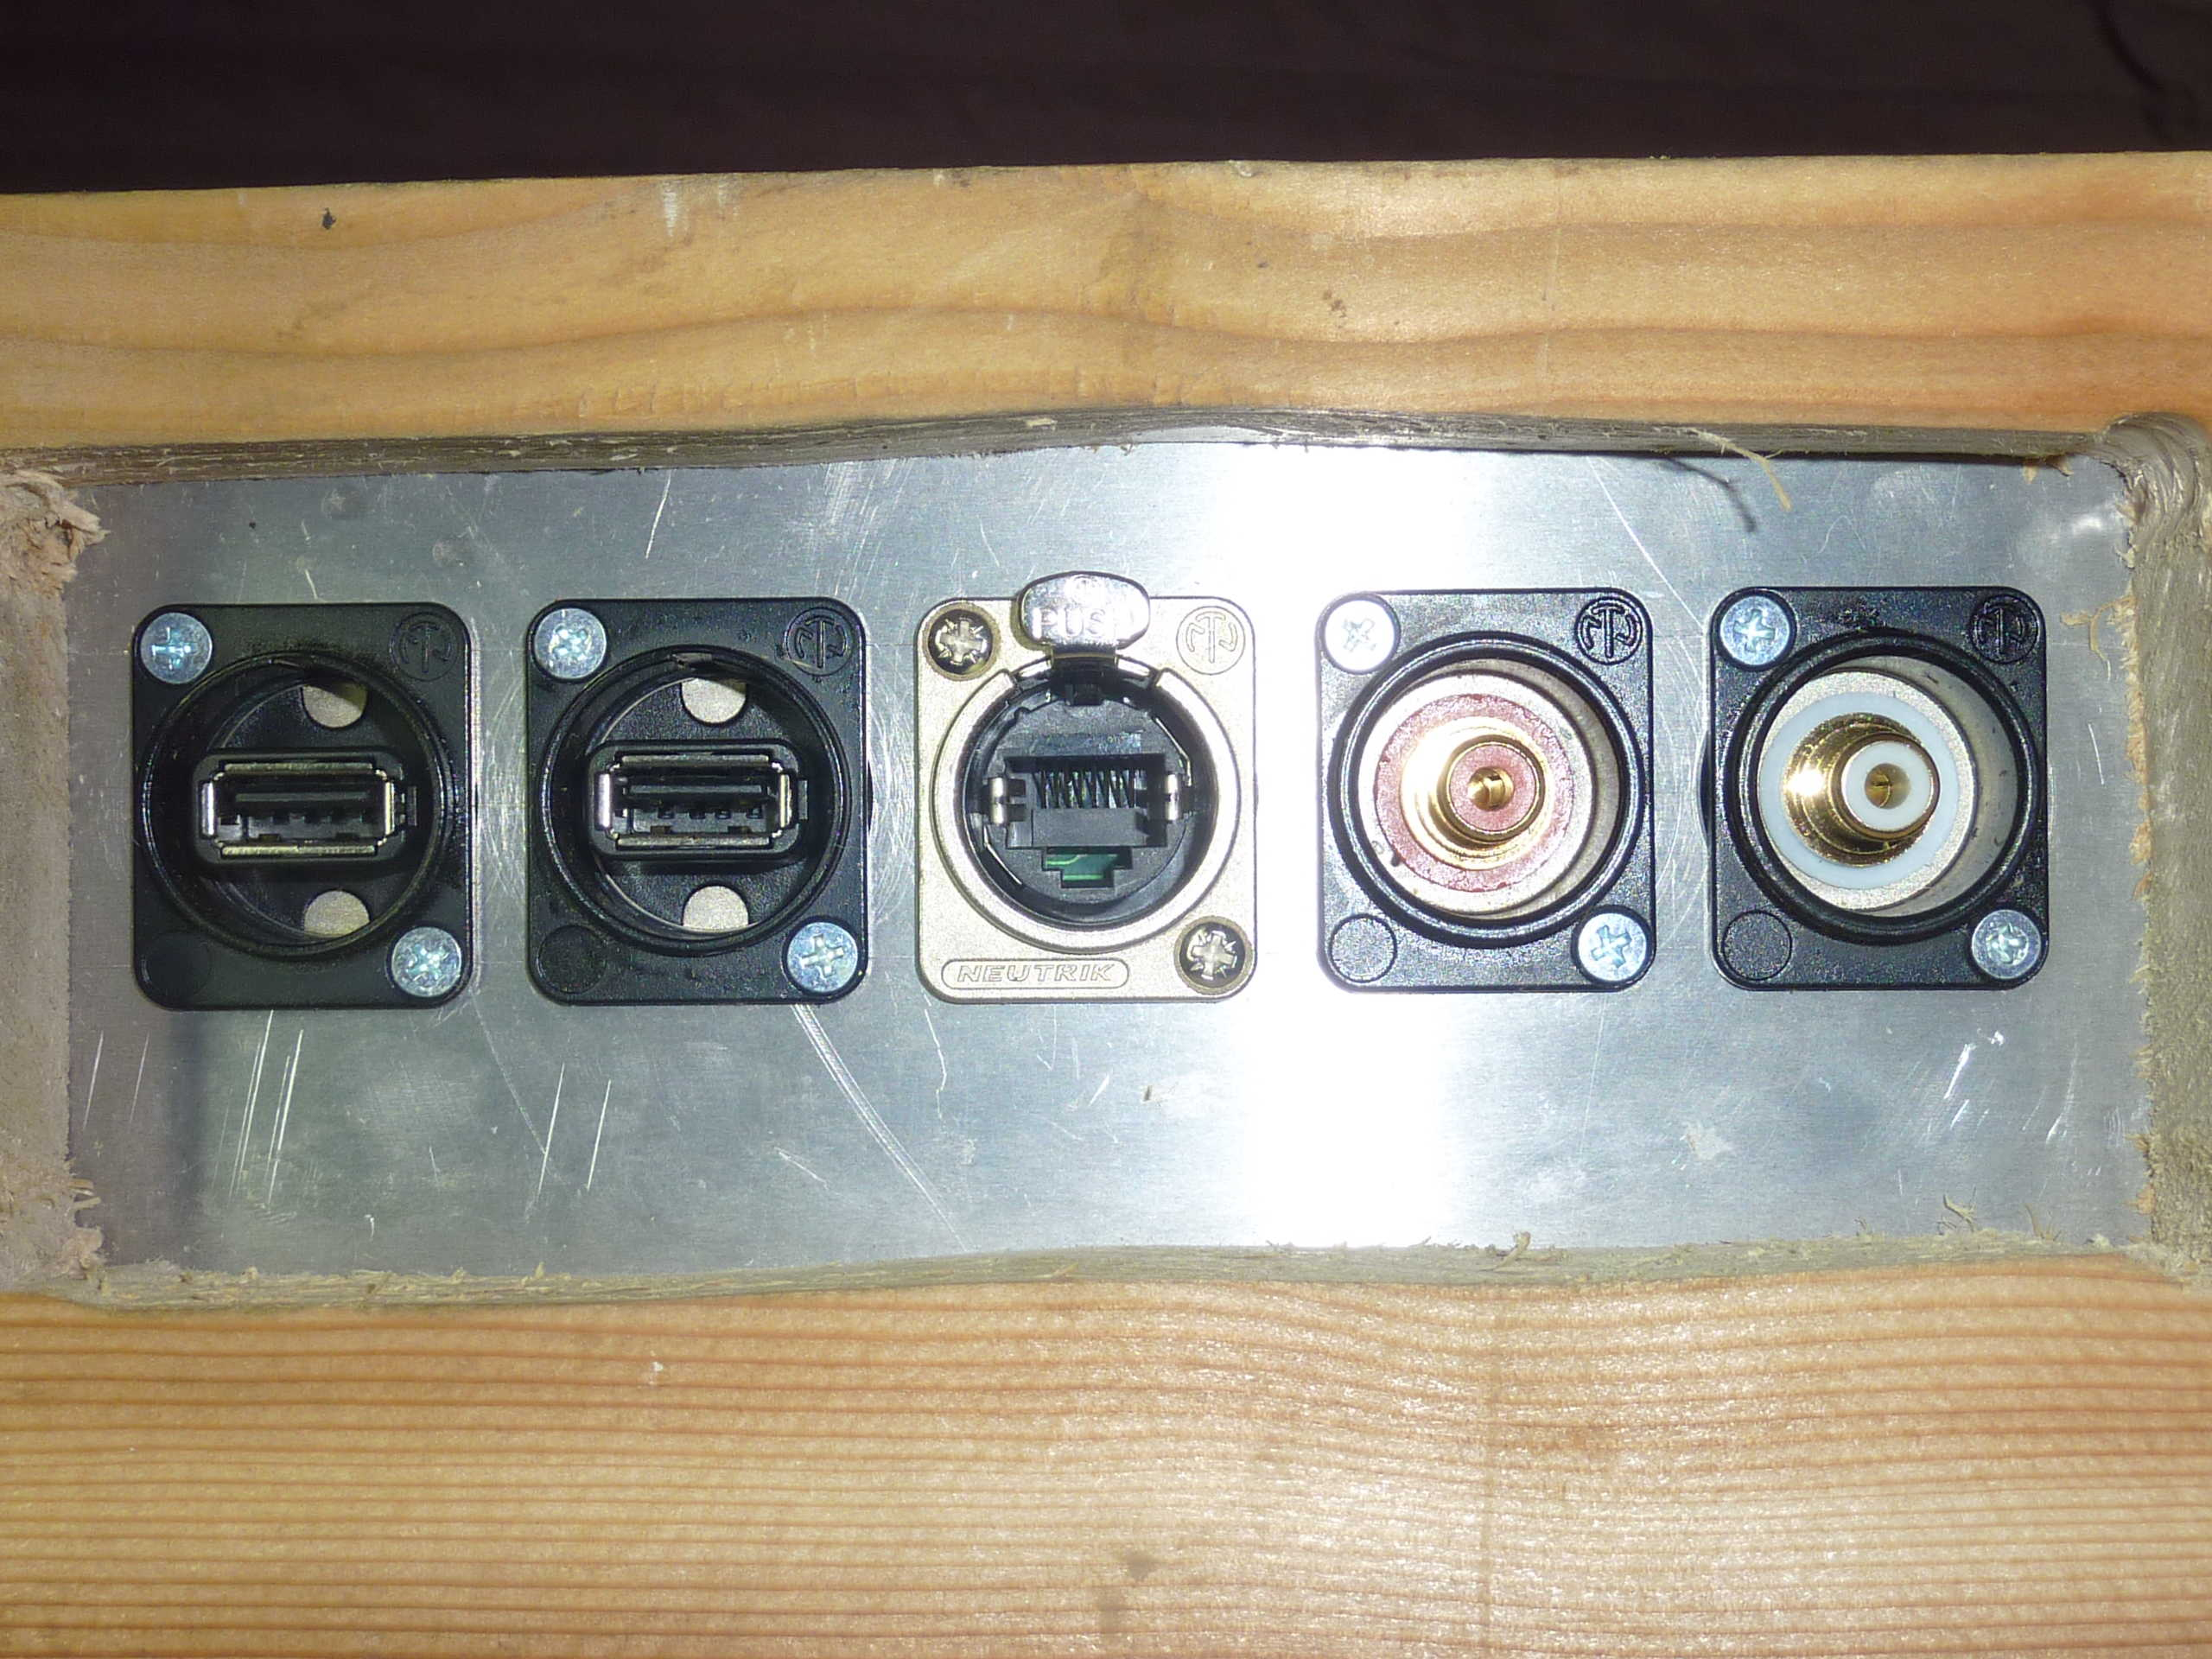
\includegraphics[width=0.8\textwidth]{RPi_YAMuPlay_Buchsen_02.JPG}
\caption{Buchsen f�r Audio, USB und LAN}
\label{fig:Buchsen}
\end{figure}

\begin{figure}[t]
\centering
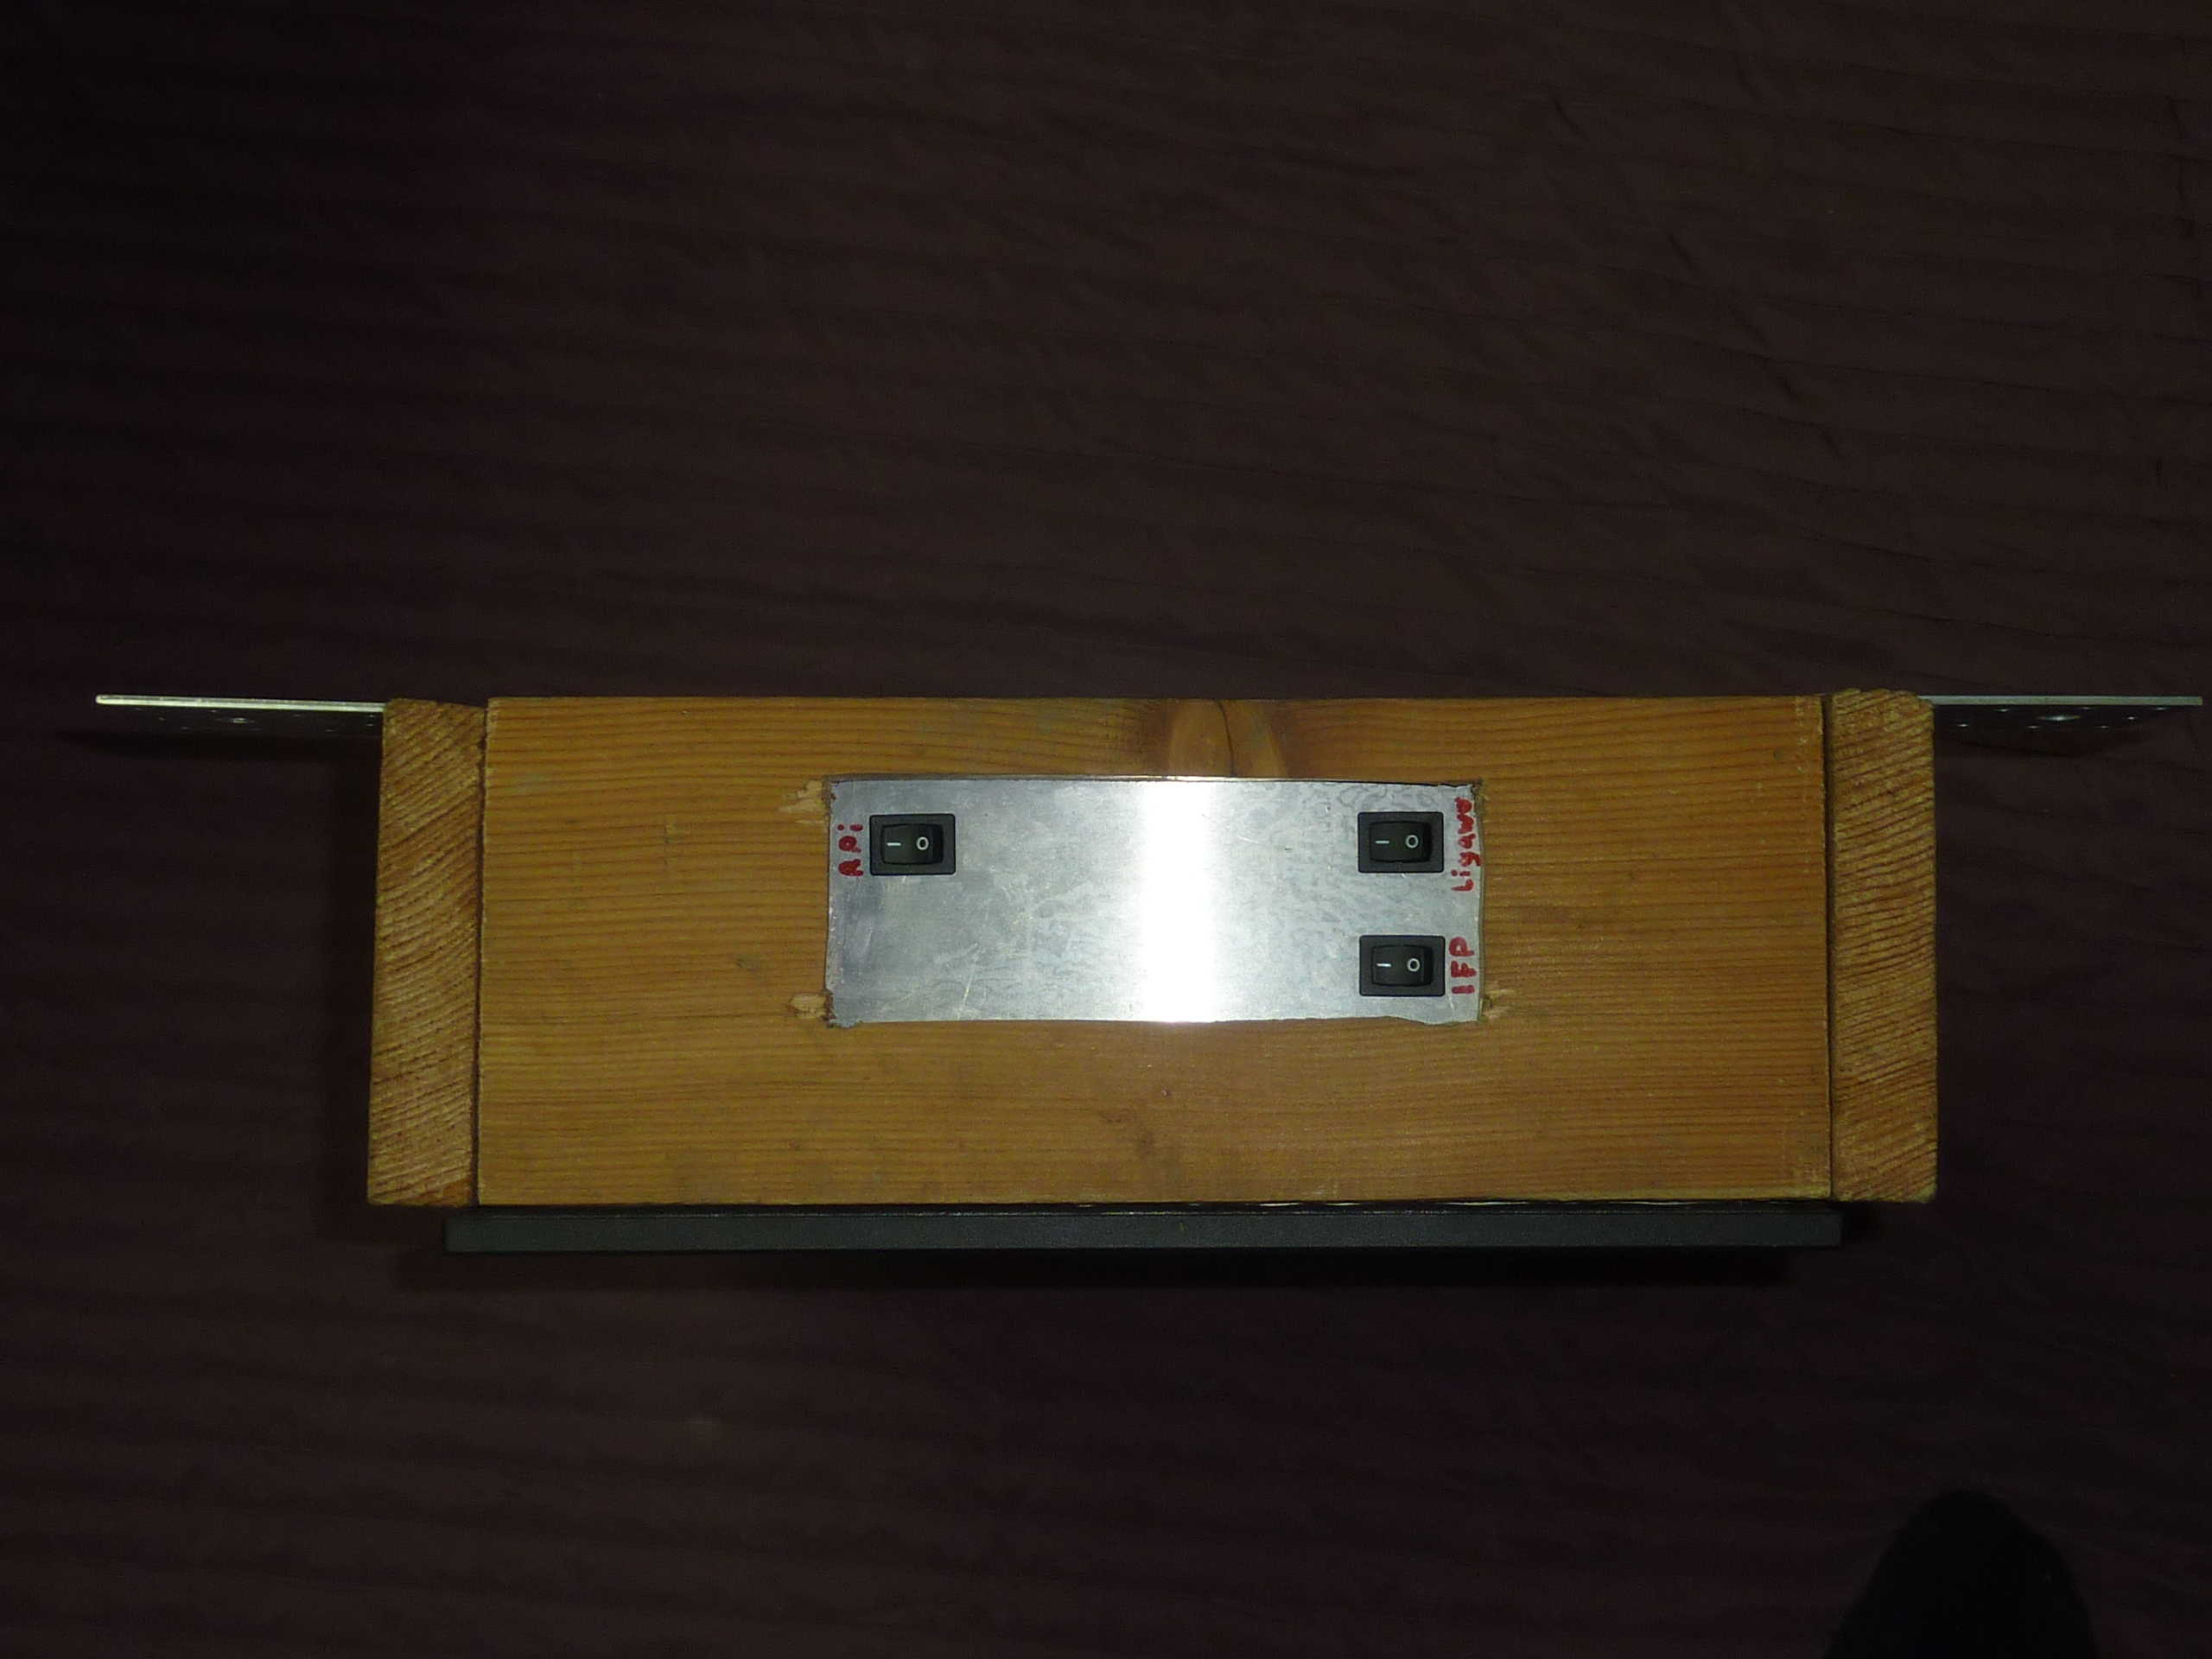
\includegraphics[width=0.8\textwidth]{RPi_YAMuPlay_Schalter.JPG}
\caption{Schalter f�r Spannungsversorgung}
\label{fig:Schalter}
\end{figure}
\clearpage


\section{Gesamtaufbau der Musikanlage auf dem Faschingswagen}
Dieser Abschnitt ist etwas "`{off topic}"', denn er behandelt keinerlei Themen
bez�glich des \RPi. Vielmehr wird hier kurz der Gesamtaufbau der Musikanlage
bestehend aus dem vorgestellten RPi-Touchpanel und klassischen
Car-Hifi-Komponenten beschrieben. Wer sich daf�r nicht interessiert, kann diesen
Teil bedenkenlos �berspringen...

Auf dem Faschingswagen wurde im Prinzip eine Car-Hifi-Anlage aufgebaut, deren
Lautst�rke und Klang jedoch nicht von einem normalen Autoradio (head unit),
sondern mit Hilfe der Frequenzweiche Sony XEC-505 gesteuert wurde. Aufgrund
der Verwendung der Software \filenam{omxplayer.bin} auf dem \RPi\ greift dort
der ALSA-Mixer nicht. Eine Lautst�rkeregelung war deshalb softwaretechnisch
nicht so leicht zu l�sen. \textit{Auch hier lasse ich mich gerne eines Besseren
belehren! \smiley{wink}} (\url{mailto:schlizbaeda@gmx.de})
Vorteilhaft an dieser L�sung war jedenfalls, dass alle Lautsprecherpaare einzeln
geregelt und ausgepegelt werden konnten.\\
Die Funktion der Sony-Frequenzweiche ist auf deren Geh�use als Blockschaltbild 
dargestellt und zwar derma�en gut, dass dieses Bild mehr sagt als 1000 Worte,
siehe Abbildung \ref{fig:Frequenzweiche_02}.

\begin{figure}[h]
\centering
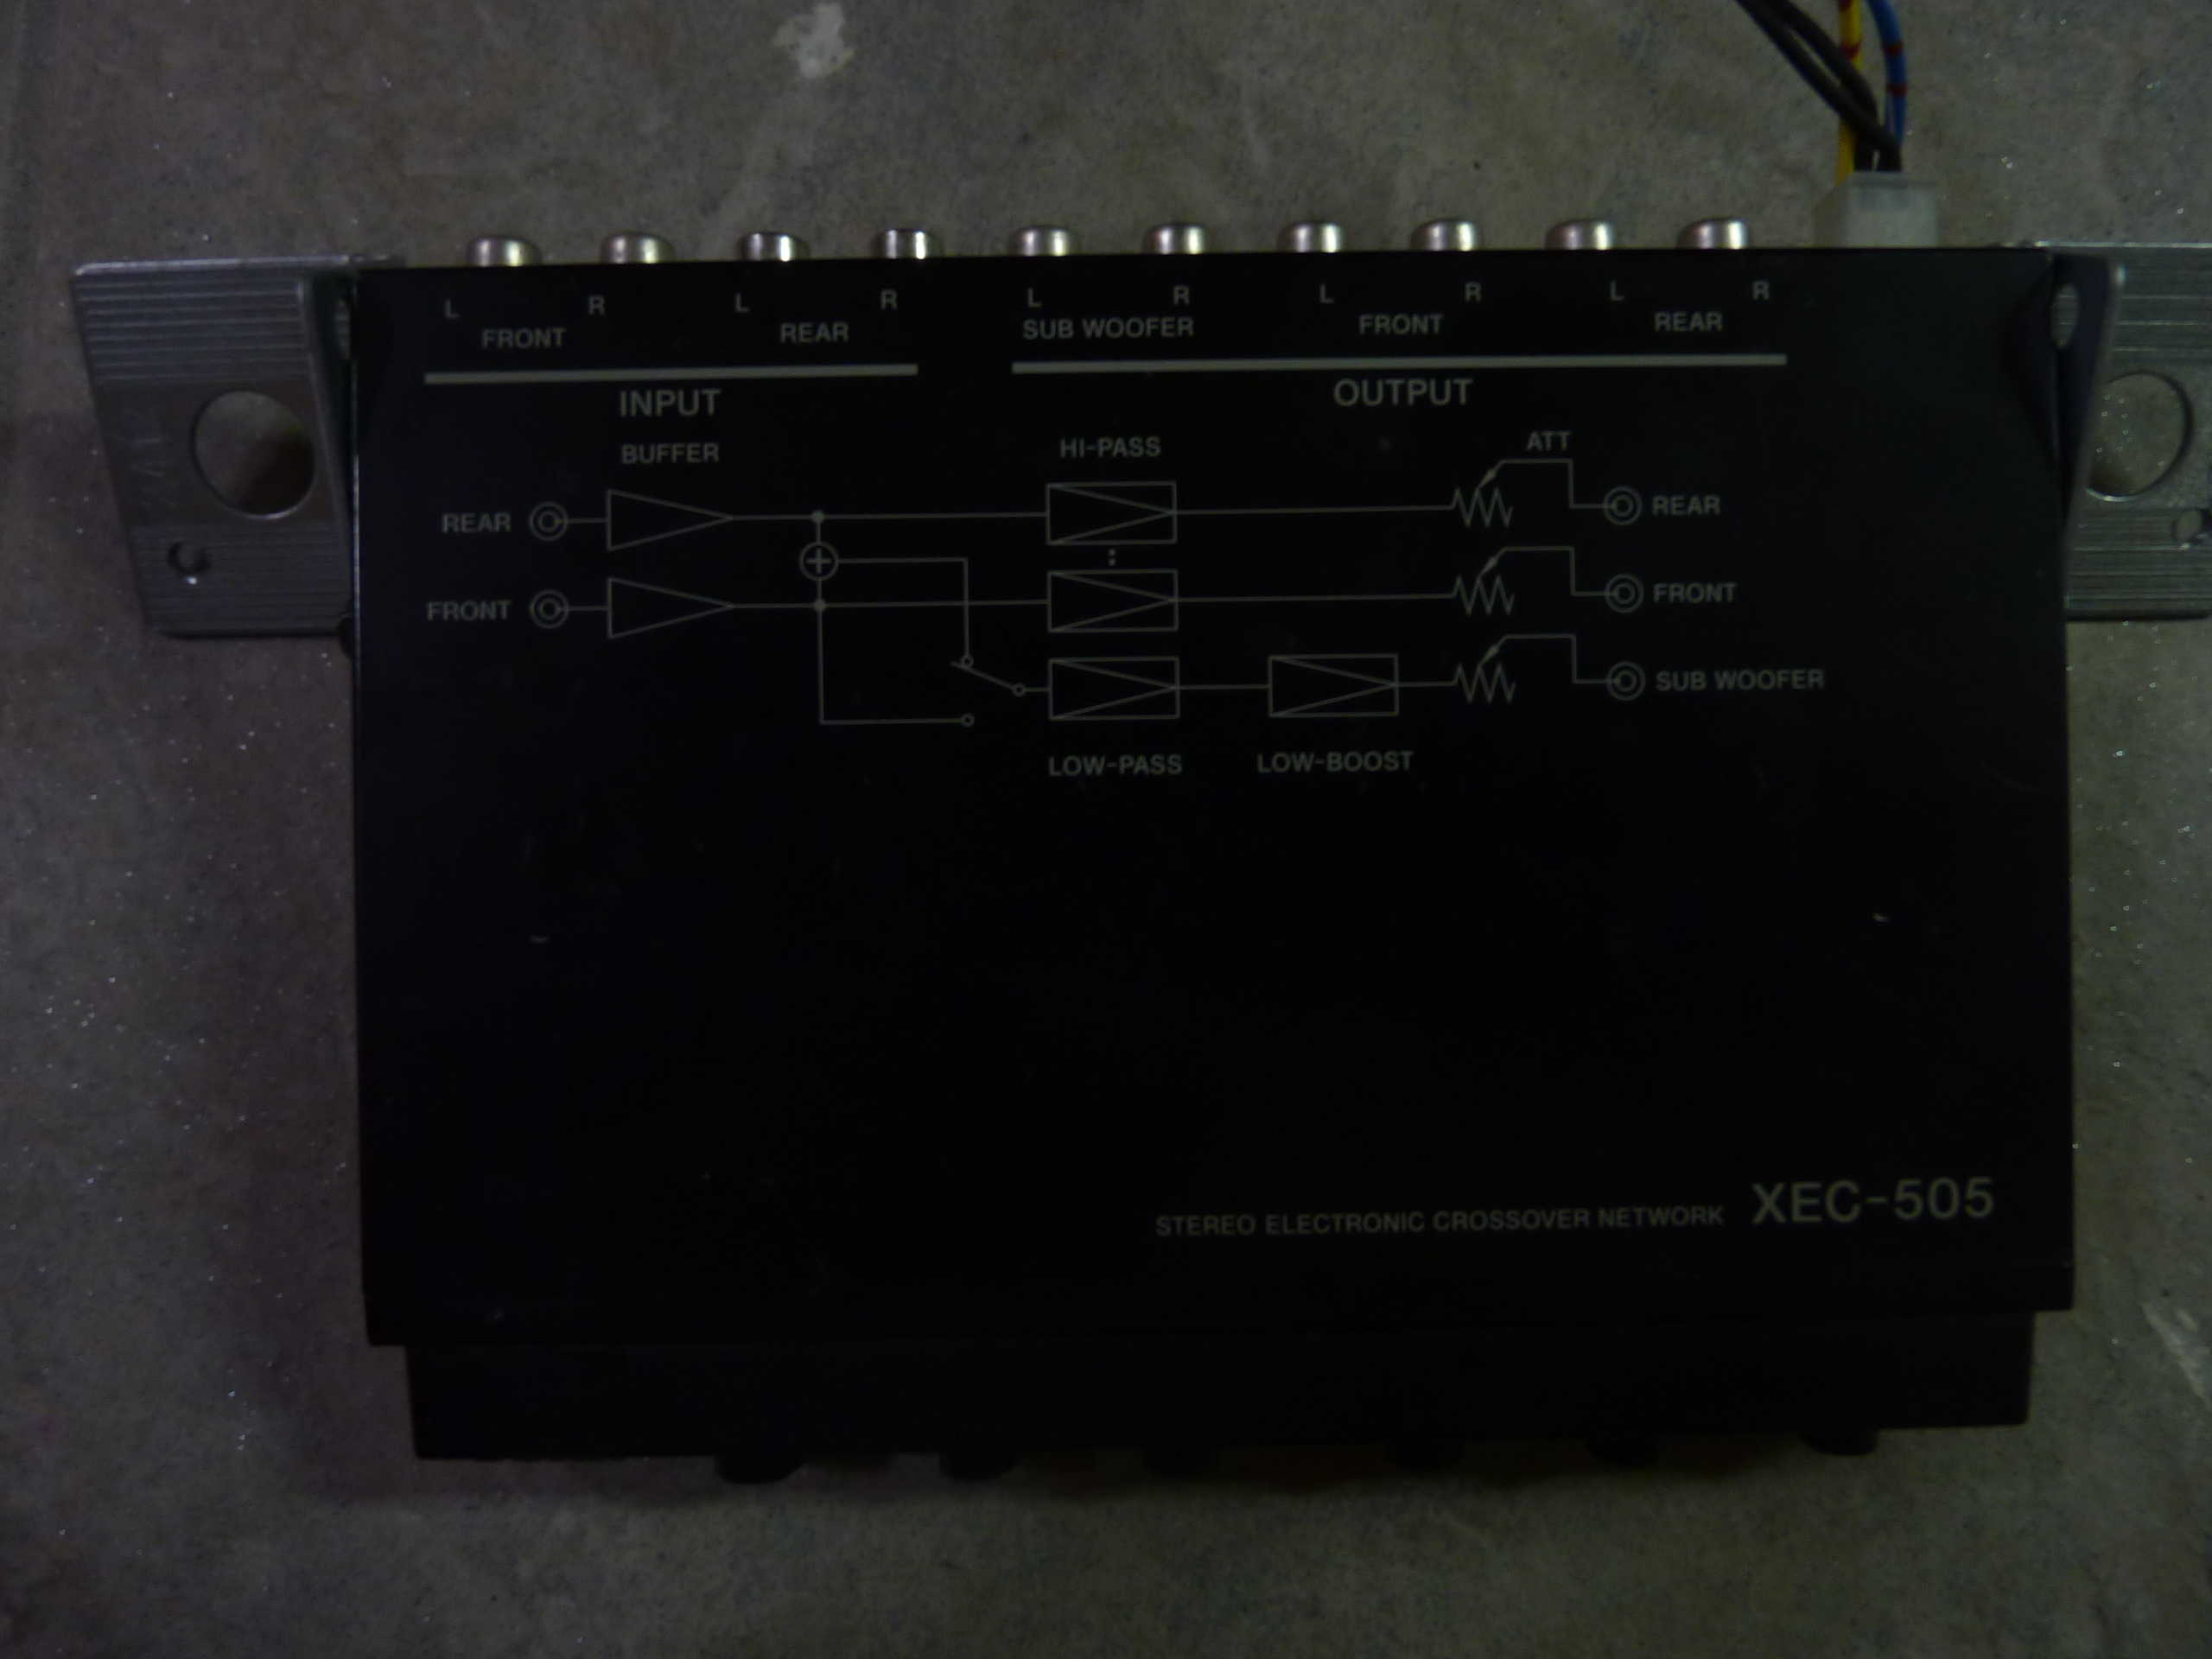
\includegraphics[width=0.9\textwidth]{Frequenzweiche_02.JPG}
\caption{Frequenzweiche}
\label{fig:Frequenzweiche_02}
\end{figure}

Aus dieser Skizze ergibt sich die Verkabelung der gesamten Musikanlage auf
Abbildung \ref{fig:Blockschaltbild_Gesamtanlage}. Es ist dann -- Achtung:
Unwort! -- \textit{nur} noch Flei�arbeit, das Ganze auf dem Faschingswagen
aufzubauen.

\begin{figure}[h]
\centering
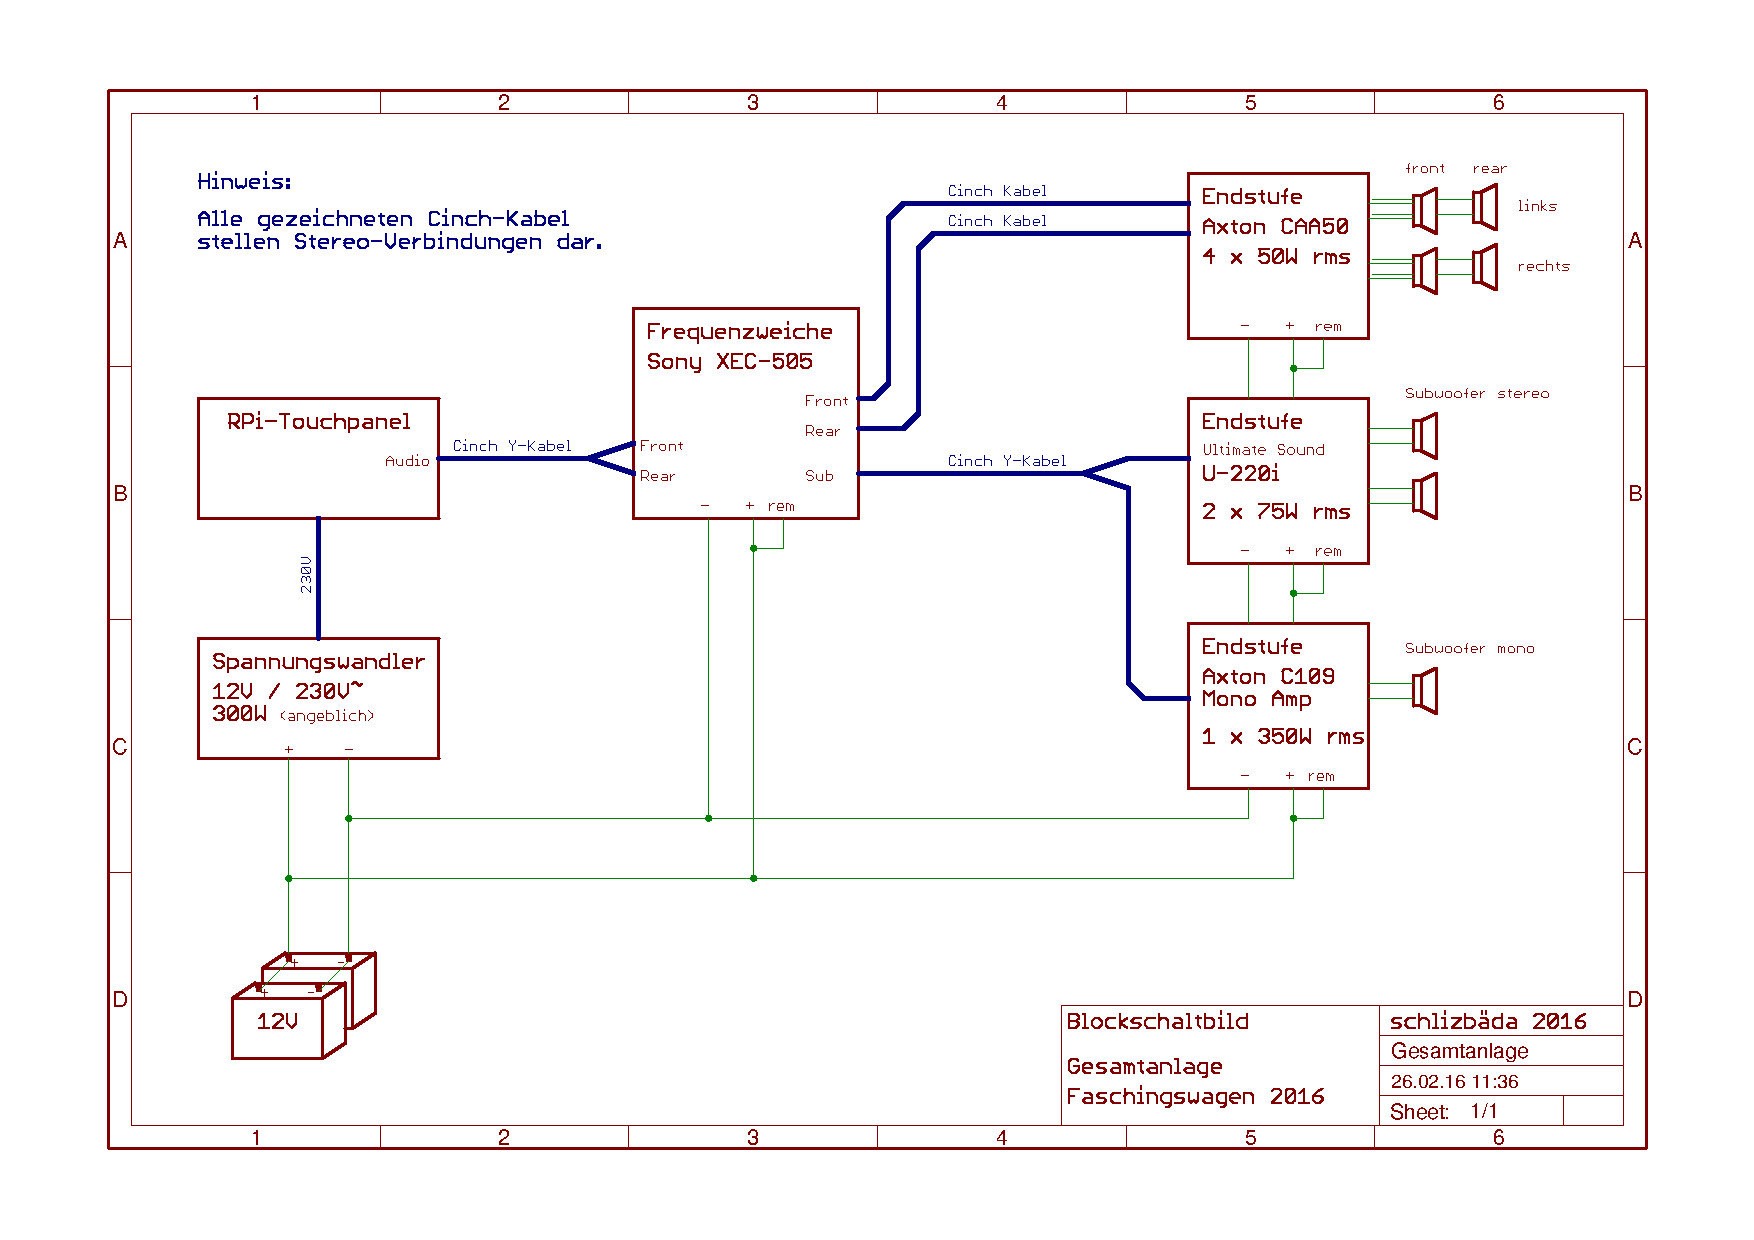
\includegraphics[width=0.9\textwidth]{Gesamtanlage.pdf}
\caption{Blockschaltbild der Musikanlage}
\label{fig:Blockschaltbild_Gesamtanlage}
\end{figure}

\begin{figure}[h]
\centering
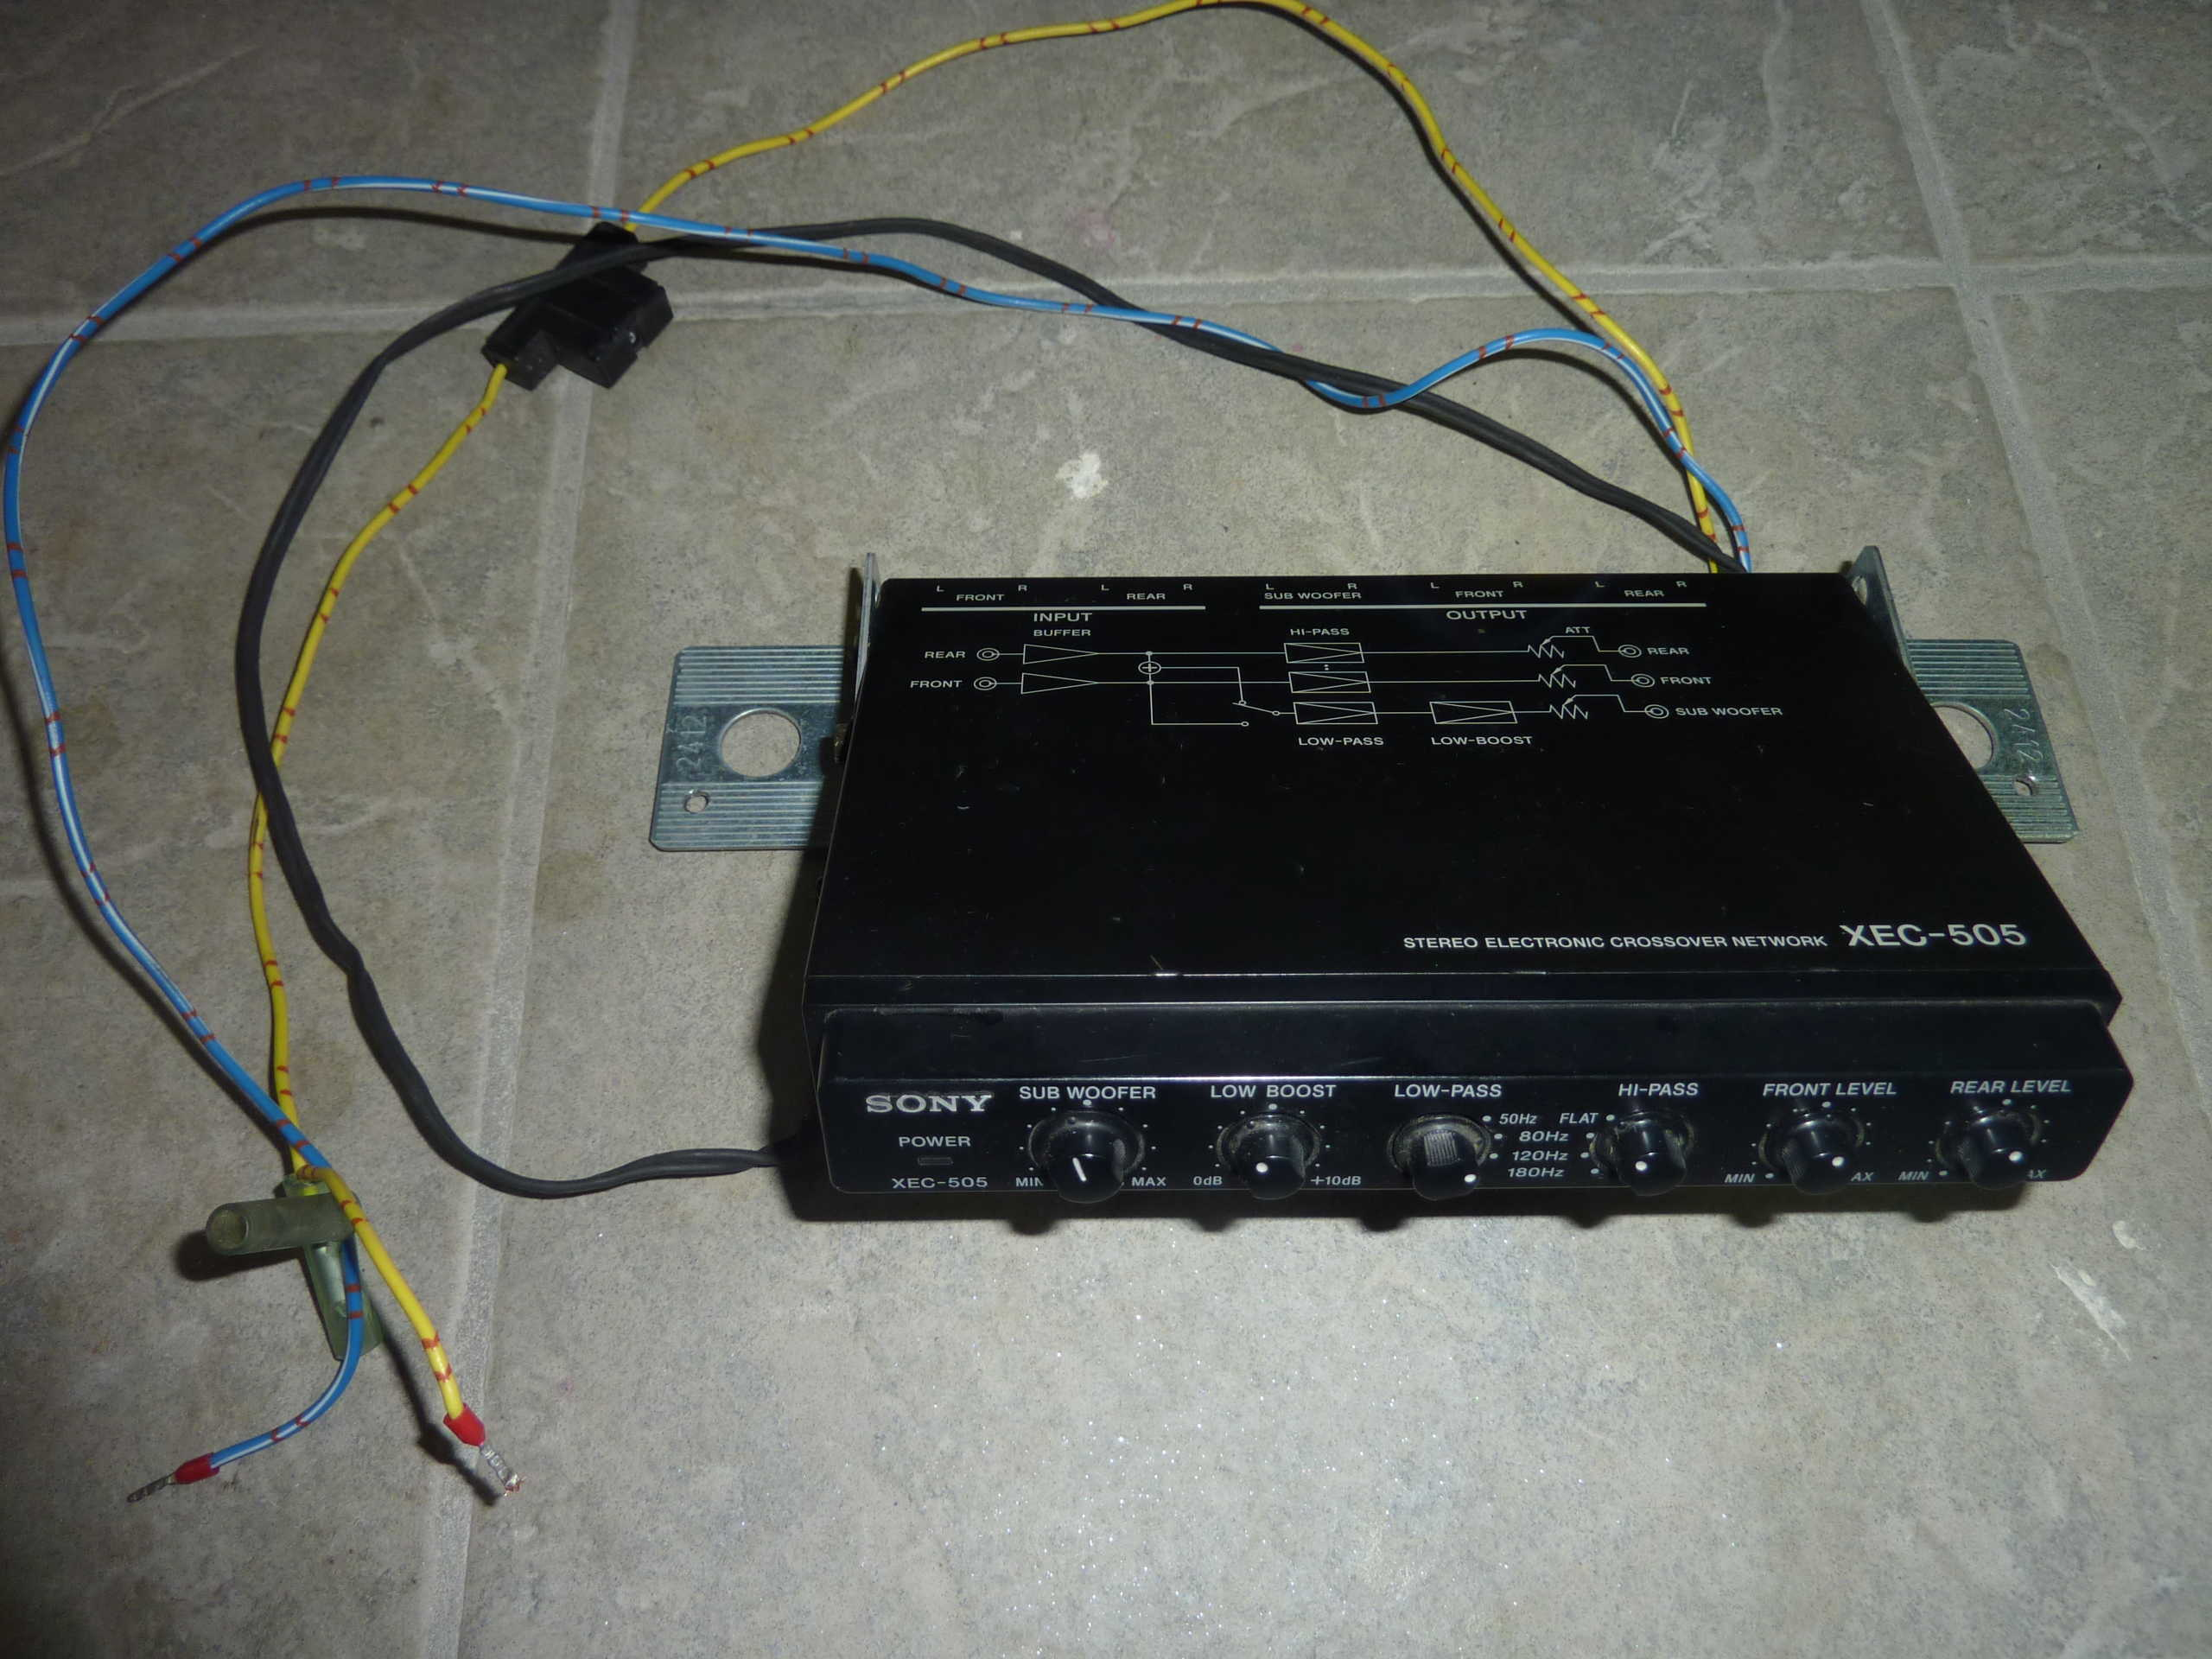
\includegraphics[width=0.9\textwidth]{Frequenzweiche_01.JPG}
\caption{Bedieneinheit der Frequenzweiche}
\label{fig:Frequenzweiche_01}
\end{figure}
\clearpage

Zuletzt noch einige Bilder vom Faschingswagen:

\begin{figure}[h]
\centering
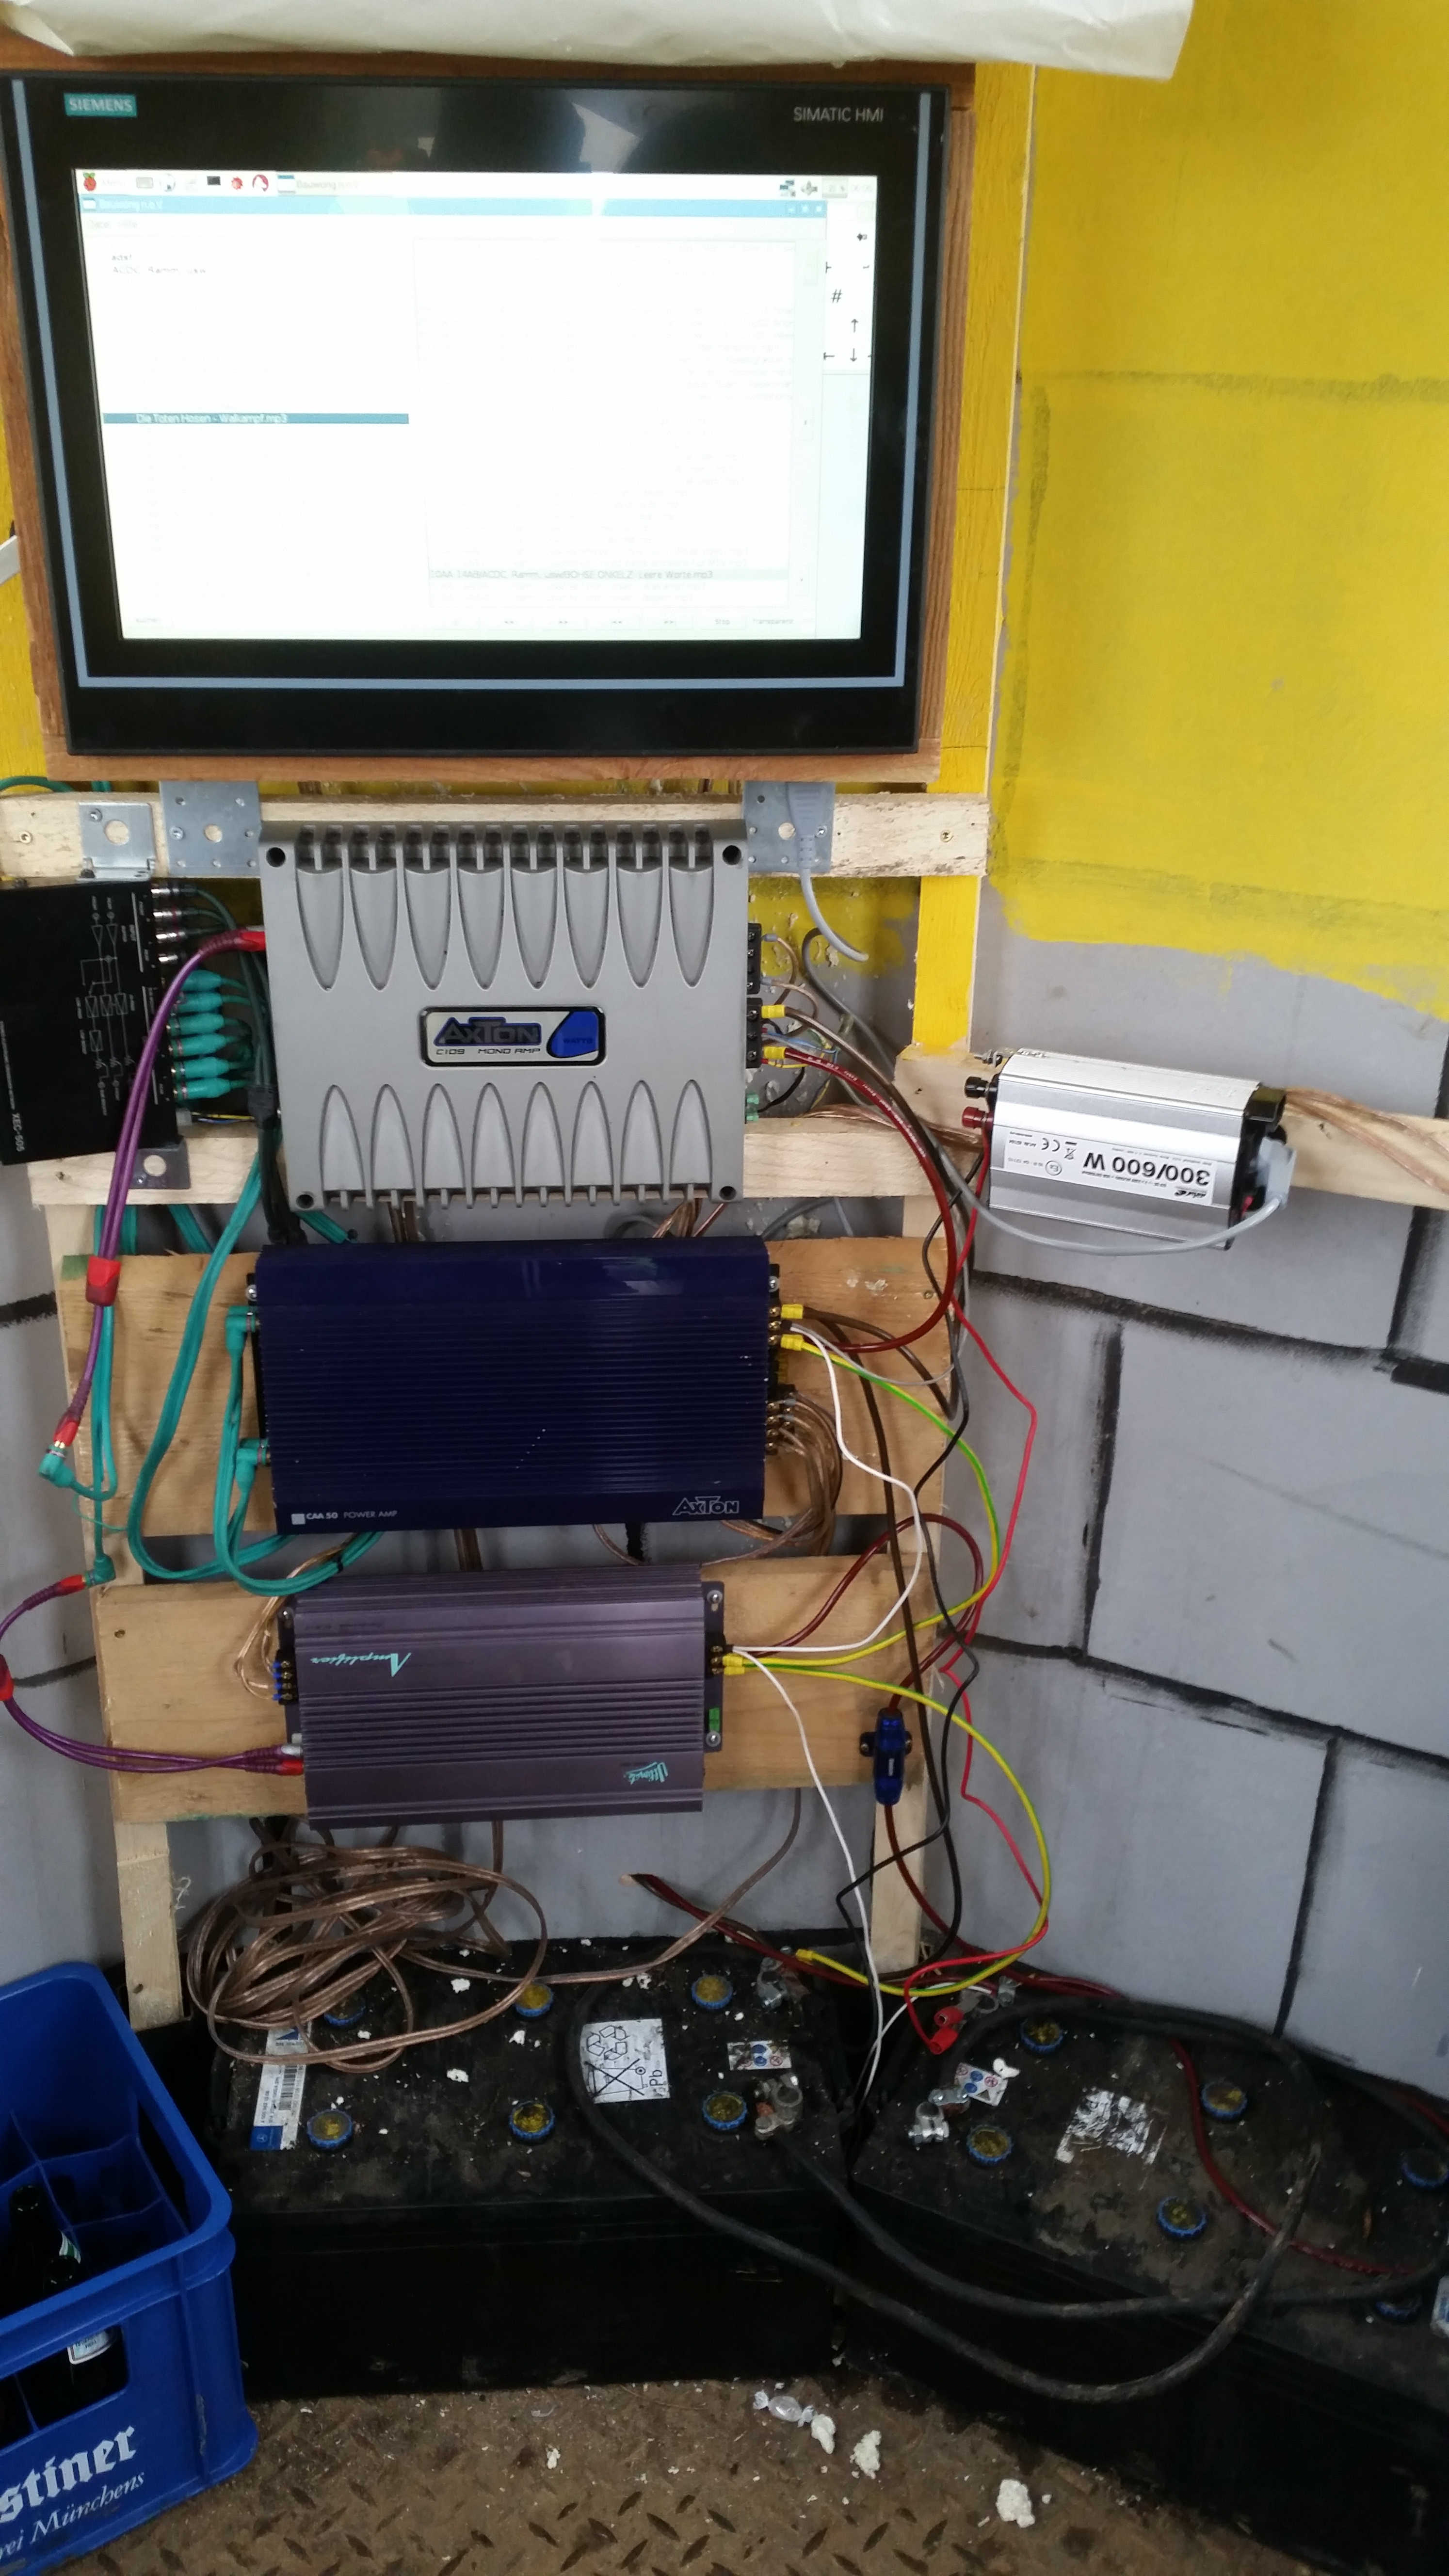
\includegraphics[width=0.63\textwidth]{Gesamtanlage.jpg}
\caption{Gesamtanlage auf dem Faschingswagen}
\label{fig:Gesamtanlage}
\end{figure}

\begin{figure}[h]
\centering
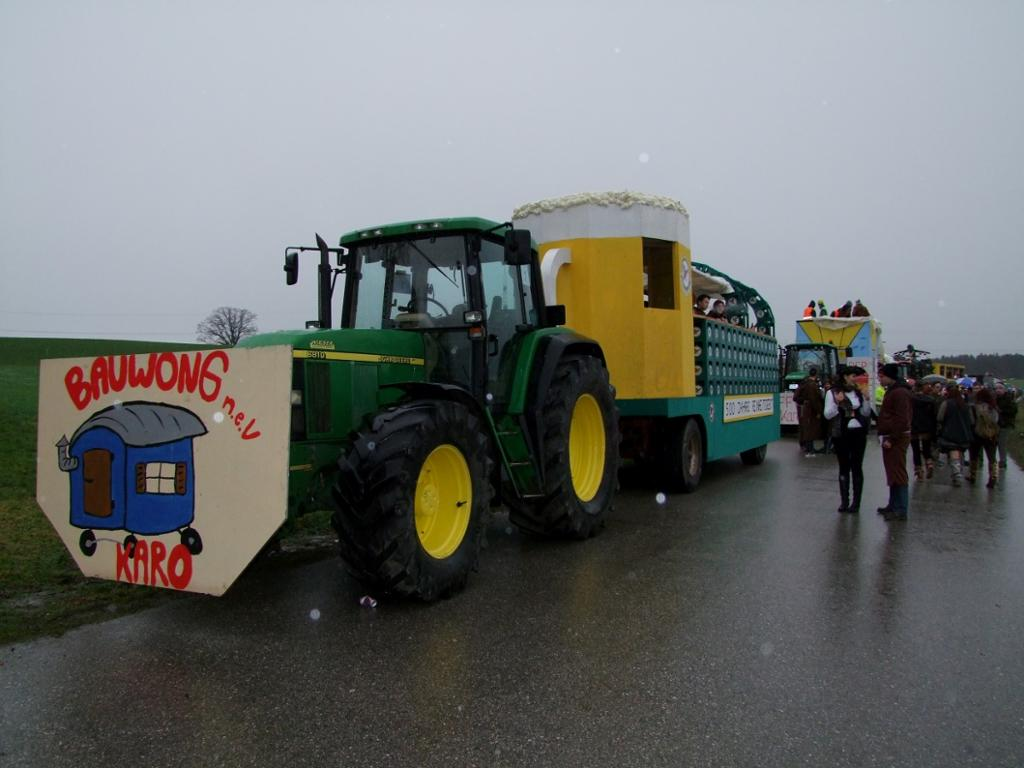
\includegraphics[width=0.8\textwidth]{Gaudiwurm_Tattenhausen_01.jpg}
\caption{18. Gaudiwurm Tattenhausen 31.01.2016 Aufstellung}
\label{fig:Tattenhausen01}
\end{figure}

\begin{figure}[h]
\centering
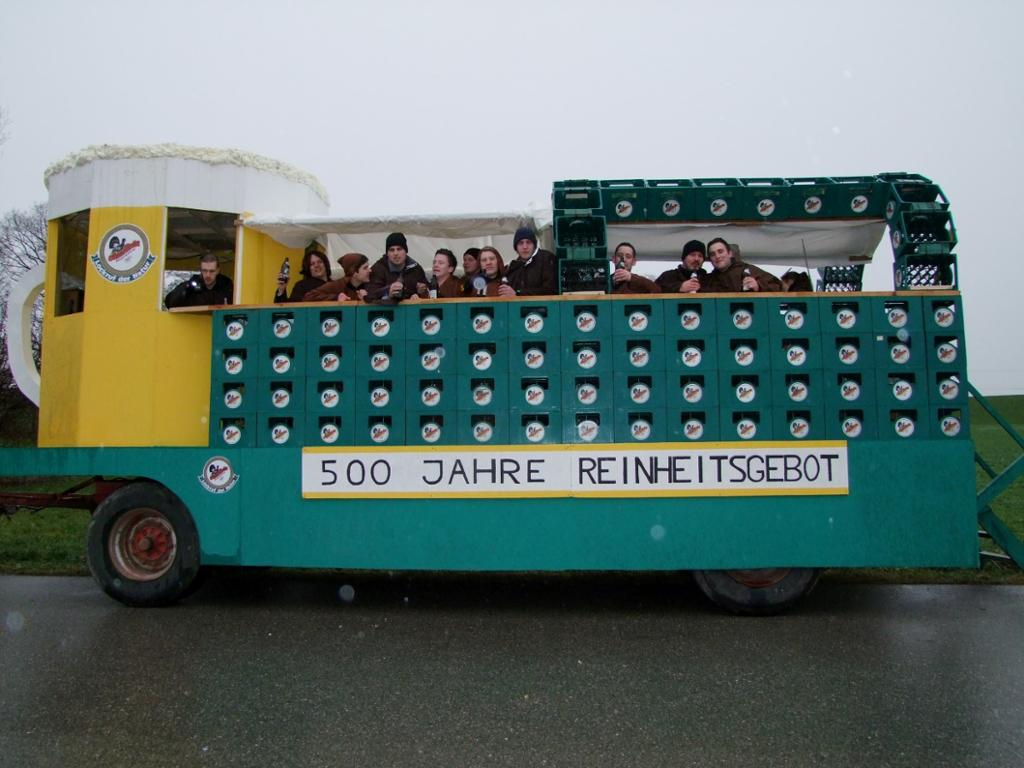
\includegraphics[width=0.8\textwidth]{Gaudiwurm_Tattenhausen_03.jpg}
\caption{18. Gaudiwurm Tattenhausen 31.01.2016 Seitenansicht}
\label{fig:Tattenhausen03}
\end{figure}
\clearpage

\begin{figure}[h]
\centering
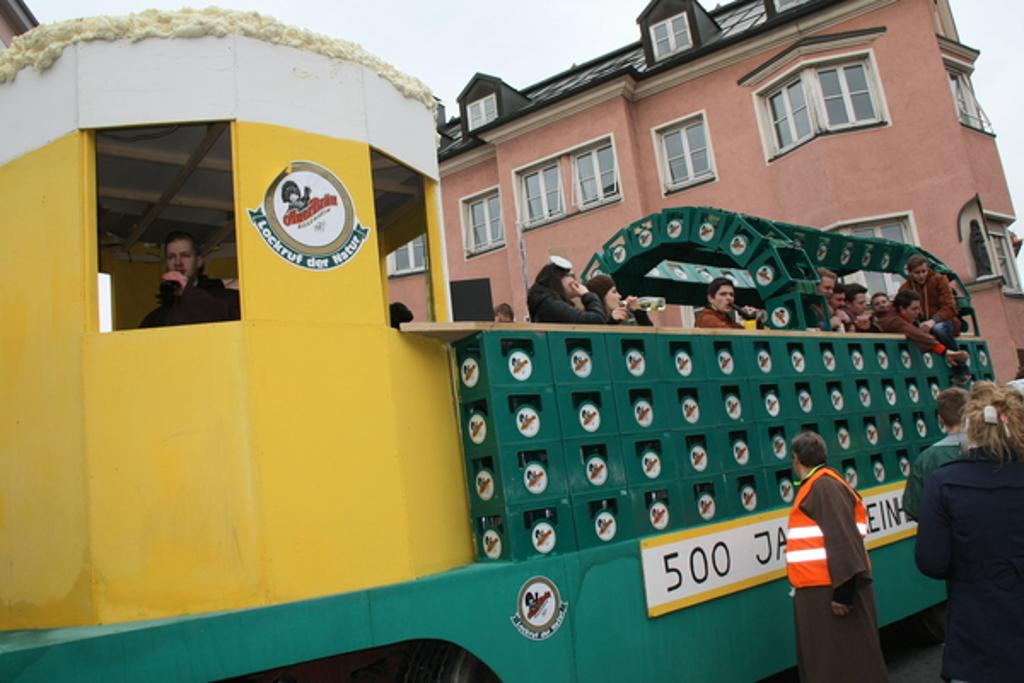
\includegraphics[width=0.8\textwidth]{Faschingszug_BadAibling_01.jpg}
\caption{Faschingszug Bad Aibling 07.02.2016}
\label{fig:BadAibling}
\end{figure}

\textbf{} % fett gedruckter :-) Leerstring, damit's das letzte Bild auf der Seite nach oben schiebt...


\chapter{Software}
\label{cha:Software}


\section{Beschreibung und Bedienung von \Bezeichnung}
Die Software \Bezeichnung\ \Version\ ist kein eigener Mediaplayer, sondern eine
Bedieneroberfl�che f�r den existierenden Kommandozeilen-Mediaplayer
{\filenam{omxplayer.bin}, der in den meisten(?) Betriebssystem-Distributionen
f�r den \RPi\ standardm��ig enthalten ist. Diese Oberfl�che ist quasi eine
"`H�lle"' -- oder auf englisch -- ein Wrapper f�r {\filenam{omxplayer.bin}. Der
Sinn f�r die Programmierung von \Bezeichnung\ lag \ua darin, eine Plattform
unter \textbf{Python3} zu schaffen, mit der man relativ einfach Mediendateien
(Musik und Videos) unter Zuhilfenahme von {\filenam{omxplayer.bin} abspielen
kann. Da \filenam{omxplayer.bin} als eigener Prozess gestartet wird und die
Kommunikation mit \Bezeichnung\ �ber \textbf{D-Bus} erfolgt, findet das
Abspielen aus der Sicht des �bergest�lpten Python-Programms im Hintergrund
statt; in Python k�nnen w�hrenddessen andere Aufgaben erledigt werden. Ein
weiterer Vorteil liegt darin, dass \filenam{omxplayer.bin} haupts�chlich den
GPU-Teil des Broadcom 2835 auf dem \RPi\ beansprucht und somit den CPU-Teil kaum
belastet. Die CPU-Last beim Betrieb von \Bezeichnung liegt bei \ca 25\%-35\%, es
bleiben gen�gend CPU-Ressourcen frei.\\
Nachteilig ist jedoch, dass ALSA aufgrund der gro�en Hardwaren�he von
\filenam{omxplayer.bin} nicht eingebunden ist und somit wirkungslos bleibt.
Daher funktioniert weder der ALSA-Mixer von Raspbian, noch kann eine Soundkarte
wie Hifiberry DAC+ eingesetzt werden. Die Audioausgabe kann nur �ber HDMI
oder den Analoganschluss des \RPi\ erfolgen, eine Laust�rkeregelung muss am
Audioverst�rker vorgenommen werden!

Es gibt bereits gen�gend kompliziert zu bedienende Mediaplayer vor allem
hinsichtlich der Erstellung, �nderung und Verwaltung von Playlists. Bereits
in Kapitel \ref{sec:Einfuehrung_Software} in der Einf�hrung habe ich die
Problematik des Music Player Daemons angedeutet. So etwas ist nicht zu
gebrauchen, wenn �nderungen \textit{schnell} vorgenommen werden sollen/m�ssen.
Vielmehr ist eine intuitive Bedieneroberfl�che erforderlich. \Bezeichnung\ ist
ein Versuch in diese Richtung, aber auch hier kann diesbez�glich noch viel
getan werden, das will ich gar nicht abstreiten. Mehrere Punkte dazu sind in
Kapitel \ref{sect:Erweiterungen} aufgef�hrt.

\begin{figure}[h]
\centering
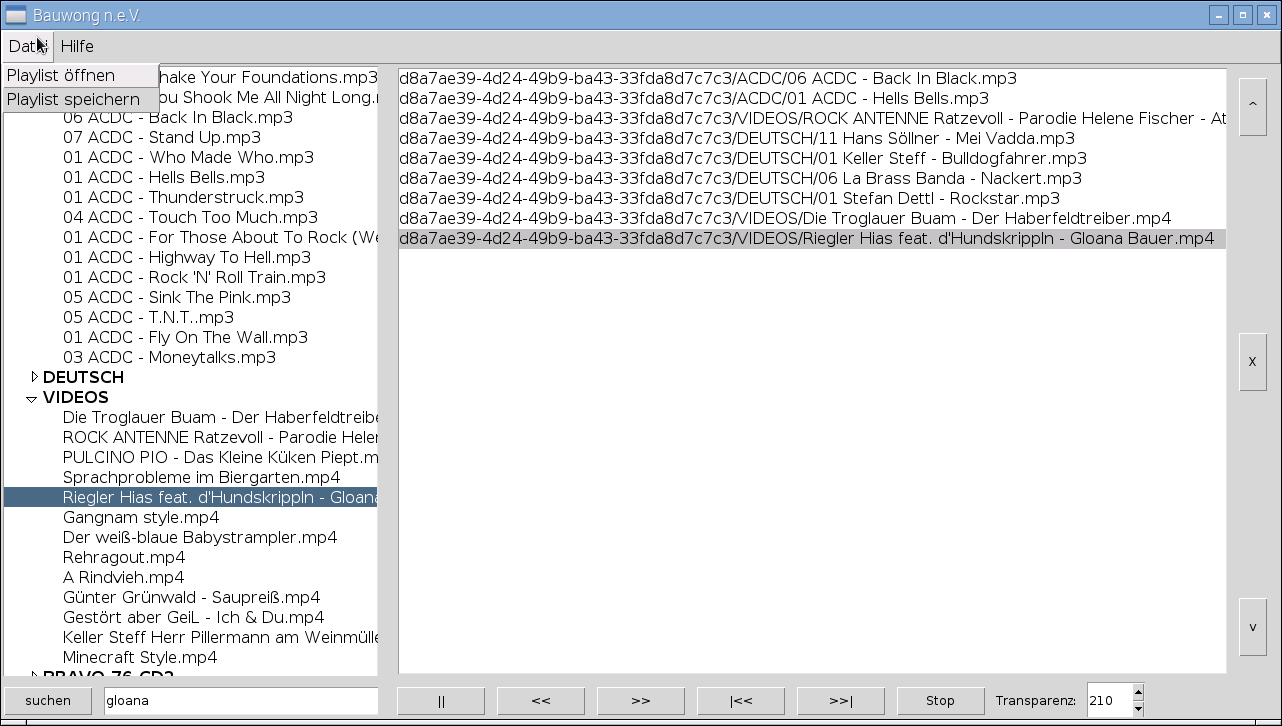
\includegraphics[width=\textwidth]{yamuplay_menu.png}
\caption{Hauptfenster von \Bezeichnung\ mit ge�ffnetem Hauptmen�}
\label{fig:yamuplay_menu}
\end{figure}

Das Hauptfenster von \Bezeichnung\ ist zweigeteilt, siehe Abbildung
\ref{fig:yamuplay_menu}. In der linken H�lfte werden alle auf den
angeschlossenen USB-Laufwerken enthaltenen Dateien und Verzeichnisse in einer
hierarchischen Baumstruktur angezeigt, gew�hnliche Dateien in Normalschrift und
Verzeichnisse in fetter Schrift. Ein Doppelklick auf ein Verzeichnis �ffnet oder
schlie�t es, eine gew�hnliche Datei wird der Playlist hinzugef�gt. Mehrmaliges
Hinzuf�gen der gleichen Datei zur Playlist ist nat�rlich m�glich. \Bezeichnung\
kann derzeit jedoch noch nicht unterscheiden, ob es sich bei der gew�hlten Datei
um eine abspielbare Mediendatei oder um einen anderen Dateityp (\zB eine
Textdatei) handelt.\\ 
Im unteren Bereich befinden sich Steuerelemente zur Dateisuche. Die Suche
ber�cksichtigt derzeit nur die \textbf{Dateinamen}, nicht die Metadaten
(\zB ID3-Tags) der Mediendateien. Dies w�rde ja eine Datenbank erfordern, auf
die aus Performancegr�nden bewusst verzichtet wurde. \\
Wird ein USB-Laufwerk entfernt oder ein weiteres angeschlossen, so wird die
Baumstruktur entsprechend aktualisiert. Dateieintr�ge in der Playlist bleiben
davon unangetastet!

Der rechte Teil enth�lt die Playlist mit den aktivierten Mediendateien. Am
rechten Rand befinden sich Schaltfl�chen, um einzelne Dateien in der Liste zu
verschieben oder wieder ganz aus der Liste zu entfernen. Unterhalb der Playlist
sind die Schaltfl�chen \textit{Play/Pause}, \textit{seek}, \textit{prev},
\textit{next} und \textit{Stop}, die den Tasten eines CD-Spielers nachempfunden
sind. Ein Doppelklick auf einen Titel in der Playlist springt sofort dorthin und
spielt diesen Titel ab.\\
Zus�tzlich ist unten ein Eingabefeld f�r die Transparenz (den sogenannten
alpha-Wert) von Videos, die zwischen 0 (vollst�ndig transparent, d.h.
unsichtbar) und 255 (vollst�ndig deckend) liegen kann. Grunds�tzlich reagiert
der Desktop auch bei deckender Anzeige von Videos auf Maus- \bzw Touchereignisse
ganz normal, die Eingabe muss allerdings "`blind"' erfolgen. Der Standardwert
von 210 f�r die Transparenz l�sst den Desktop des \RPi\ und \Bezeichnung\ noch
leicht durchscheinen, so dass eine Bedienung m�glich ist.

�ber das Men� von \Bezeichnung\ k�nnen in der Leiste \menuitem{Datei} Playlists
geladen und gespeichert werden. Es wird der Standarddialog des Betriebssystems
zur Dateiauswahl angezeigt, mit dem der Dateiname festgelegt werden kann. Das
Dateiformat ist \Code{m3u}, eine Textdatei, in der jede Zeile eine Mediendatei
enth�lt. Beim Abspeichern einer Playlist werden immer \textbf{alle} Elemente der
Playlist in die Datei geschrieben, beim Laden werden alle Eintr�ge der Datei an
die aktuell bestehende Playlist \textbf{hinten angeh�ngt}.

\begin{figure}[h]
\centering
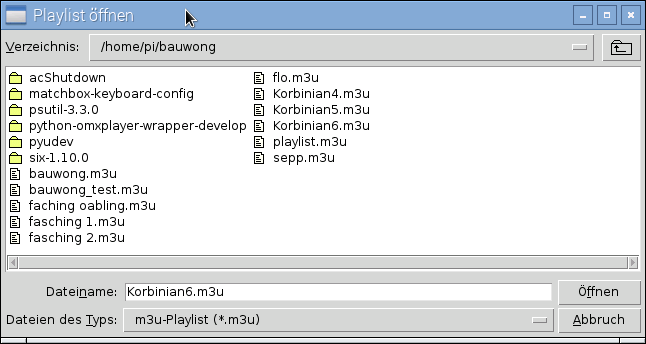
\includegraphics[width=0.6\textwidth]{yamuplay_open.png}
\caption{Dateidialog von \Bezeichnung\ zum Laden einer vorhandenen Playlist}
\label{fig:yamuplay_open}
\end{figure}

Der Men�punkt \menuitem{Hilfe\arrowright Info} zeigt eine sogenannte
"`About-Box"' an, in der Informationen �ber die Software und die Lizenz
angezeigt werden, siehe \ref{fig:yamuplay_about}.

\begin{figure}[h]
\centering
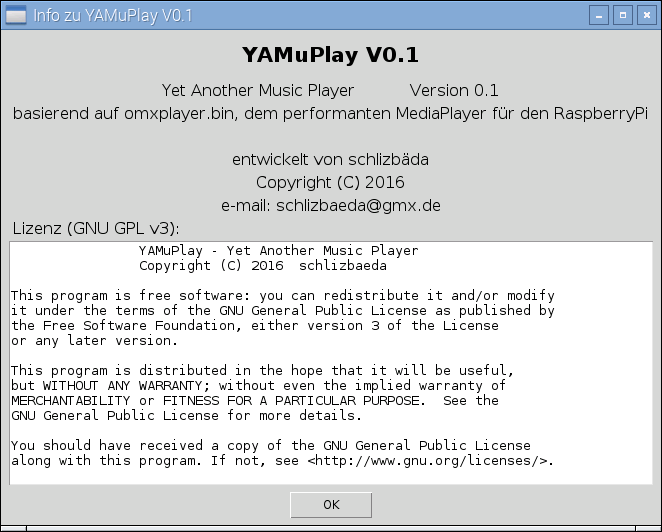
\includegraphics[width=0.75\textwidth]{yamuplay_about.png}
\caption{About-Box von \Bezeichnung}
\label{fig:yamuplay_about}
\end{figure}

\begin{bclogo}[logo = \bclampe, noborder = true]{Hinweis}
Da am Ende die Zeit davonlief (ich wei�, eine schlechte Ausrede \smiley{wink}),
wurde die gesamte grafische Oberfl�che von \Bezeichnung\ f�r eine Displaygr��e
von 1366x768 Pixeln "`optimiert"', d.h. es wird von einer Fensterh�he von ca.
720 Pixeln ausgegangen. Die Breite ist unkritischer.
\end{bclogo}
\clearpage


\section{Bibliotheken und Module}
Zur Installation von \Bezeichnung\ ben�tigt man folgende Bibliotheken und Module:

\begin{table}[!h]
\centering
\renewcommand{\arraystretch}{1.5}
\begin{tabular}{|l|l|l|p{0.45\textwidth}|}
\toprule[2pt]
\textbf{Modul} & \textbf{Version} & \textbf{Lizenz} & \textbf{Quelle}\\
\midrule[2pt]
\Code{python3-pip} & aktuell(?) & MIT-Lizenz & \Code{apt-get install python\textbf{3}-pip}\\
\midrule[2pt]
\Code{python-omxplayer-wrapper} & 0.0.2 & LGPL v3 & \url{https://github.com/willprice/python-omxplayer-wrapper}\\
\hline
\Code{python3-dbus} & 1.2.2-1 & MIT-Lizenz & \Code{apt-get install python3-dbus}\\
\hline
\Code{pyudev} & 0.18 & LGPL v2.1 & \url{https://github.com/pyudev}\\
\hline
\Code{six} & 1.10.0 & MIT-Lizenz & \url{https://pypi.python.org/pypi/six}\\
\midrule[2pt]
\Code{\matchboxKeyboard} & aktuell(?) & LGPL v... & \url{https://github.com/mwilliams03/matchbox-keyboard.git}\\
%\hline
\bottomrule[2pt]
\end{tabular}
\vspace{0.5cm}
\caption{In \Bezeichnung\ eingebundene Bibliotheken und Module}
\label{tab:Bibliotheken}
\end{table}

\begin{bclogo}[logo = \bclampe, noborder = true]{Hinweis}
Die Tabelle \ref{tab:Bibliotheken} ist eine Liste aller notwendigen Module,
die zur Ausf�hrung von \Bezeichnung\ erforderlich sind. \textbf{Bitte jetzt
noch nicht die in der Spalte "`Quelle"' angegebenen Download-Kommandos
ausf�hren!}  Sie dienen nur dem vorl�ufigen �berblick. Eine
Schritt-f�r-Schritt-Anleitung erfolgt im folgenden Kapitel \ref{sect:Install}.
\end{bclogo}

\Bezeichnung\ selbst ben�tigt f�r seinen Betrieb nur die Module
\Code{python-omxplayer-wrapper}, \Code{python3-dbus}, \Code{pyudev} und
\Code{six}. Das Modul \Code{python\textbf{3}-pip} muss auf dem \RPi\ installiert
werden, damit die vier genannten Python-Module wiederum richtig installiert
werden k�nnen.\\
Die Software \Code{\matchboxKeyboard} ist nur dann notwendig, wenn keine
reale Tastatur verwendet werden soll, so wie auf dem Faschingswagen.
 

\section{Installation von \Bezeichnung\ auf dem \RPi}
\label{sect:Install}
Dieser Abschnitt beschreibt die \textbf{vollst�ndige} Installation von
\Bezeichnung\ auf einem jungfr�ulichen Raspbian-System mit dem Ausgabestand
\textit{wheezy} vom 05.05.2015, Imagedatei\\
\filenam{2015-05-05-raspbian-wheezy.img}.\\
Ich habe die Beschreibung m�glichst detailliert gehalten, damit alle Leser die
Sache durch- und nachvollziehen k�nnen, egal auf welchem Erfahrungsstand sie
sich befinden. An den beschrieben Punkten hatte ich anfangs als grimmiger Linux-
und Python-Noob selbst meine Probleme!\\
Grunds�tzlich kann diese Installationsanleitung in f�nf Bereiche aufgegliedert
werden:
\begin{itemize}
\item Raspbian-Image auf eine SD-Karte (4GB oder gr��er) aufspielen und updaten
\item \filenam{/boot/config.txt} anpassen
\item \Bezeichnung\ und alle notwendigen Python-Module installieren
\item Desktop des \RPi\ einrichten
\item Touchpanel-Tastatur \textit{\matchboxKeyboard} installieren
\end{itemize}

\begin{bclogo}[logo = \bclampe, noborder = true]{Hinweis}
F�r die Installation muss der \RPi\ zwingend einen Internetzugang erhalten.\\
Zudem sollten zumindest am Anfang Tastatur und Maus angeschlossen sein. Die
Interaktion mit dem \RPi\ kann im sp�teren Verlauf der Inbetriebnahme wahlweise
auch �ber \Code{ssh} erfolgen.
\end{bclogo}


\subsection{Raspbian-Image auf eine 4GB SD-Karte aufspielen und updaten}
Die gesamte Installation wurde auf \textit{raspbian wheezy}, Ausgabestand
05.05.2015 durchgef�hrt. Mittlerweile ist die Nachfolgeversion
\textit{jessie} ver�ffentlicht, mit der die Installation ebenso funktionieren
sollte.\\
In dieser Anleitung wird davon ausgegangen, dass ein aktuelles Raspbian-Image
auf die SD-Karte aufgespielt wurde und das allererste, automatisch startende
\Code{raspi-config} bereits abgeschlossen wurde. Ferner ist vom \RPi\ aus eine
Internetverbindung verf�gbar. \textbf{Wenn alle diese Bedingungen erf�llt sind,
kann ab jetzt auch mit \Code{ssh} gearbeitet werden.}

\begin{itemize}
\item \textbf{\Code{raspi-config} ausf�hren}\\
      \Code{sudo raspi-config}\\
      Men�punkt \Code{1 Expand Filesystem} ausf�hren, um Platz f�r die Backups w�hrend der System-Updates zu schaffen\\
      Spracheinstellungen im Men�punkt \Code{4 Internationalisation Options} durchf�hren
\item \textbf{Raspbian-Update ohne Kernel und Broadcom-Firmware durchf�hren}\\
      \Code{sudo apt-get update}\\
      \Code{sudo apt-get dist-upgrade}
\item \textbf{Kernel- und Broadcom-Firmware-Update durchf�hren}\\
      \begin{bclogo}[logo = \bclampe, noborder = true]{Hinweis}
      Das hier beschriebene Kernel- und Firmwareupdate war bei meiner
      urspr�nglichen \textit{wheezy}-Installation erforderlich. Beim aktuellen
      \textit{jessie}-Image sollte es nicht mehr notwendig sein. Generell birgt
      jedes Kernel- und Firmware-Update in sich das Risiko, neue Probleme zu
      verursachen und sollte m�glichst vermieden werden.
      \end{bclogo}

      \Code{uname -a} \# liefert die aktuelle Kernel-Version, \zB:\\
      \prompt{Linux raspberrypi 3.18.11+ #781 PREEMPT Tue Apr 21 18:02:18 BST 2015 armv6l GNU/Linux}\\
      \Code{vcgencmd version} \# liefert die aktuelle Firmware-Version, \zB:\\
      \prompt{Apr 21 2015 14:42:19\\
              Copyright (c) 2012 Broadcom\\
              version 2d5ad04b63af4233440c3f7c8587108223201102 (clean) (release)}\\
      Update durchf�hren:\\
      \Code{sudo apt-get install rpi-update}\\
      \Code{sudo rpi-update}\\
      \Code{sudo reboot}\\
      Update kontrollieren:\\
      \Code{uname -a}\\
      \prompt{Linux raspberrypi 4.1.18+ #845 Thu Feb 18 19:37:13 GMT 2016 armv6l GNU/Linux}\\
      \Code{vcgencmd version}\\
      \prompt{Feb 25 2016 18:51:26\\
              Copyright (c) 2012 Broadcom\\
              version dea971b793dd6cf89133ede5a8362eb77e4f4ade (clean) (release)}
\end{itemize}


\subsection{\filenam{/boot/config.txt} anpassen}
Bei Verwendung der Hardwarekomponente \textbf{\Ligawo} wird empfohlen, die
HDMI-Einstellungen in der Datei \filenam{/boot/config.txt} anzupassen.

\begin{itemize}
\item \textbf{Unterst�tzte Aufl�sungen des angeschlossenen Bildschirms ermitteln}\\
      \Code{tvservice --modes=CEA} \# ermittelt die unterst�tzen Modi f�r die HDMI-Gruppe CEA (Consumer Electronics Association)\\
      \Code{tvservice --modes=DMT} \# ermittelt die unterst�tzen Modi f�r die HDMI-Gruppe DMT (Display Monitor Timing)\\
      \begin{figure}[h]
      \centering
      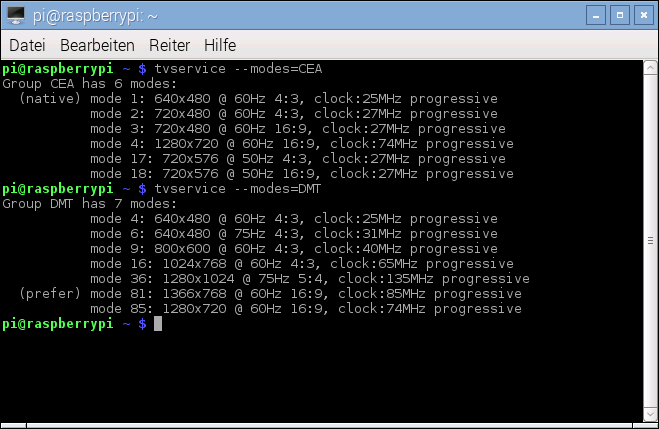
\includegraphics[width=0.9\textwidth]{tvservice.png}
      \caption{Ausgaben des Kommandos \Code{tvservice}}
      \label{fig:tvservice}
      \end{figure}
      \\Den beiden Ausgaben kann man die optimale Aufl�sung entnehmen:
      Im Beispiel aus Abbildung \ref{fig:tvservice} handelt es sich um den Modus 81 aus der HDMI-Gruppe DMT
\newpage
\item \textbf{Editieren der Datei \filenam{/boot/config.txt}}\\
      Eintrag \Code{hdmi\_group=2} \# CEA = Gruppe 1 / DMT = Gruppe 2\\
      Eintrag \Code{hdmi\_mode=81} \# 1366x768 Pixel\\
      Eintrag \Code{hdmi\_drive=2} \# Audio-Signal �ber HDMI erzwingen\\
      In Abbildung \ref{fig:config_txt} sind die Anpassungen f�r das verwendete 19-Zoll Siemens Industrial Flat Panel gezeigt.
      \begin{figure}[h]
      \centering
      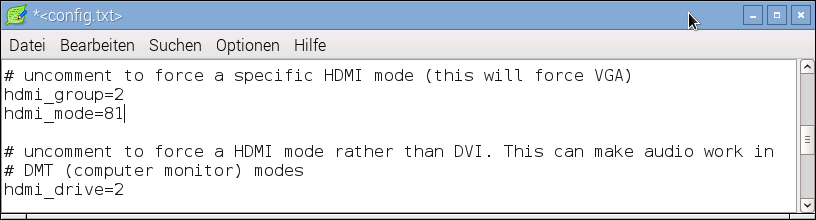
\includegraphics[width=0.9\textwidth]{config_txt.png}
      \caption{�nderungen in der Datei \filenam{/boot/config.txt}}
      \label{fig:config_txt}
      \end{figure}
\item \textbf{\Code{raspi-config} ausf�hren}\\
      \Code{sudo raspi-config}\\
      Men�punkt \Code{8 Advanced Options} ausf�hren\\
      Es �ffnet sich ein Untermen�:\\
      Men�punkt \Code{A9 Audio} �ffnen und Option \Code{2 Force HDMI} w�hlen
\end{itemize}


\subsection{\Bezeichnung\ und alle notwendigen Python-Module installieren}
\begin{itemize}
\item \textbf{Package Installer f�r Python3 installieren}\\
      \Code{sudo apt-get install python3-pip}\\
      Es wird das \Code{pip}-Installationsprogramm f�r Python3-Module installiert.
\item \textbf{GitHub-Download des Python-Moduls \Code{python-omxplayer-wrapper}}\\
      \Code{cd /home/pi}\\
      Die Original-Software wurde f�r Python2.x erstellt (\url{https://github.com/willprice/python-omxplayer-wrapper}). Um es f�r Python3 anzupassen habe ich auf GitHub einen sogenannten \textit{Fork} angelegt, eine Projektabspaltung. Download und Entpacken in das Unterverzeichnis \filenam{python-omxplayer-wrapper} mit\\
      \Code{git clone https://github.com/schlizbaeda/python-omxplayer-wrapper.git}\\
      \Code{cd python-omxplayer-wrapper}\\
      Das folgende Kommando f�r den \textit{Package Installer f�r Python3} �bernimmt die aktuelle Version des Moduls in die Python3-Bibliothek. Dieser Aufruf ist immer notwendig, wenn �nderungen an diesem Modul gemacht wurden!\\
      \Code{sudo python3 setup.py install}\\
      \Code{sudo apt-get install python3-dbus} \# notwendig f�r die DBus-Kommunikation des Wrappers mit \filenam{omxplayer.bin}
\item \textbf{GitHub-Download des Python-Moduls \Code{pyudev}}\\
      Dieses Modul wird f�r die \textit{Plug-and-Play}-Erkennung am USB-Anschluss ben�tigt. Verwendung von Version 0.19 oder h�her:\\
      \Code{cd /home/pi}\\
      \Code{git clone https://github.com/pyudev/pyudev.git}\\
      \Code{cd pyudev}\\
      \Code{sudo python3 setup.py install}
\item \textbf{GitHub-Download von \Code{\Bezeichnung}}\\
      \textit{\textbf{\Bezeichnung} ist derzeit auf GitHub noch unter dem Projektnamen (Repository) \Code{bauwong} abgelegt!}\\
      \Code{cd /home/pi}\\
      \Code{git clone https://github.com/schlizbaeda/bauwong.git}\\
      \Code{cd bauwong}\\
      \Code{chmod a+x bauwong.py} \# Die Python-Programmdatei ausf�hrbar machen
\end{itemize}
%%%%%%%%%%  Alte Version %%%%%%%%%%
%\subsection{\Bezeichnung\ und alle notwendigen Python-Module installieren}
%\begin{itemize}
%\item \textbf{Package Installer f�r Python3 installieren}\\
%      \Code{sudo apt-get install python3-pip}\\
%      Es wird das \Code{pip}-Installationsprogramm f�r Python3-Module installiert
%\item \textbf{Verzeichnis \filenam{/home/pi/bauwong} anlegen}\\
%      \Code{mkdir /home/pi/bauwong}
%\item \textbf{\Code{python-omxplayer-wrapper-develop} installieren}\\
%      \Code{cd /home/pi/bauwong}\\
%      \Code{sudo git clone https://github.com/willprice/python-omxplayer-wrapper.git} \# Download und Entpacken im aktuellen Verzeichnis\\
%      \Code{cd python-omxplayer-wrapper}\\
%      Es sind Anpassungen f�r Python3 in den beiden Dateien \filenam{build/lib/omxplayer/bus\_finder.py} und \filenam{build/lib/omxplayer/player.py} notwendig!\\
%      \Code{sudo python3 setup.py install} \# Dieses Kommando des \textit{Package Installers f�r Python3} �bernimmt die aktuelle Version des Moduls von \filenam{/home/pi/bauwong} in die Python3-Bibliothek. Dieser Aufruf ist immer notwendig, wenn �nderungen an diesem Modul �bernommen werden sollen!\\
%      \Code{sudo apt-get install python3-dbus} \# notwendig f�r die D-Bus-Kommunikation des Wrappers mit \filenam{omxplayer.bin}.
%\item \textbf{\Code{pyudev} installieren}\\
%      \Code{cd /home/pi/bauwong}\\
%      \Code{sudo git clone https://github.com/lunaryorn/pyudev.git} \# Download und Entpacken im aktuellen Verzeichnis\\
%      \Code{cd pyudev}\\
%      Es sind Anpassungen f�r Python3 in der Dateien \filenam{src/pyudev/glib.py} notwendig!\\
%      \Code{sudo python3 setup.py install} \# Dieses Kommando des \textit{Package Installers f�r Python3} �bernimmt die aktuelle Version des Moduls von \filenam{/home/pi/bauwong} in die Python3-Bibliothek. Dieser Aufruf ist immer notwendig, wenn �nderungen an diesem Modul �bernommen werden sollen!\\
%      Modul \Code{six} installieren:\\
%      * Download der Datei \filenam{six-1.10.0.tar.gz} von \url{https://pypi.python.org/pypi/six}\\
%      * \Code{cd /home/pi/bauwong}\\
%      * \Code{tar xvf six-1.10.0.tar.gz}\\
%      * \Code{cd six-1.10.0}\\
%      * \Code{sudo python3 setup.py install}
%\end{itemize}

\begin{bclogo}[logo = \bclampe, noborder = true]{Es ist so weit!}
Jetzt ist der Zeitpunkt gekommen, die neu installierte Software
\textbf{\Bezeichnung} auszuprobieren \smiley{smile}. Geben Sie dazu im
Terminalfenster bitte folgende Kommandos ein:\\
\Code{cd /home/pi/bauwong} \textit{\# Da sollten Sie sich bereits befinden!}\\
\Code{./bauwong.py}\\
Es sollte die grafische Oberfl�che von \Bezeichnung\ aus Abbildung
\ref{fig:yamuplay_menu} gestartet werden. Nun muss nur noch ein USB-Memorystick
mit Musikdateien angesteckt werden und es kann losgehen!
\end{bclogo}


\subsection{Desktop des \RPi\ einrichten}
Nachdem die Software nun l�uft, kann der Desktop des \RPi\ etwas
benutzerfreundlicher eingerichtet werden \smiley{smile}. Im GitHub-Repository
befinden sich im Unterverzeichnis \filenam{desktop} daf�r vorbereitete Dateien.

\begin{figure}[h]
\centering
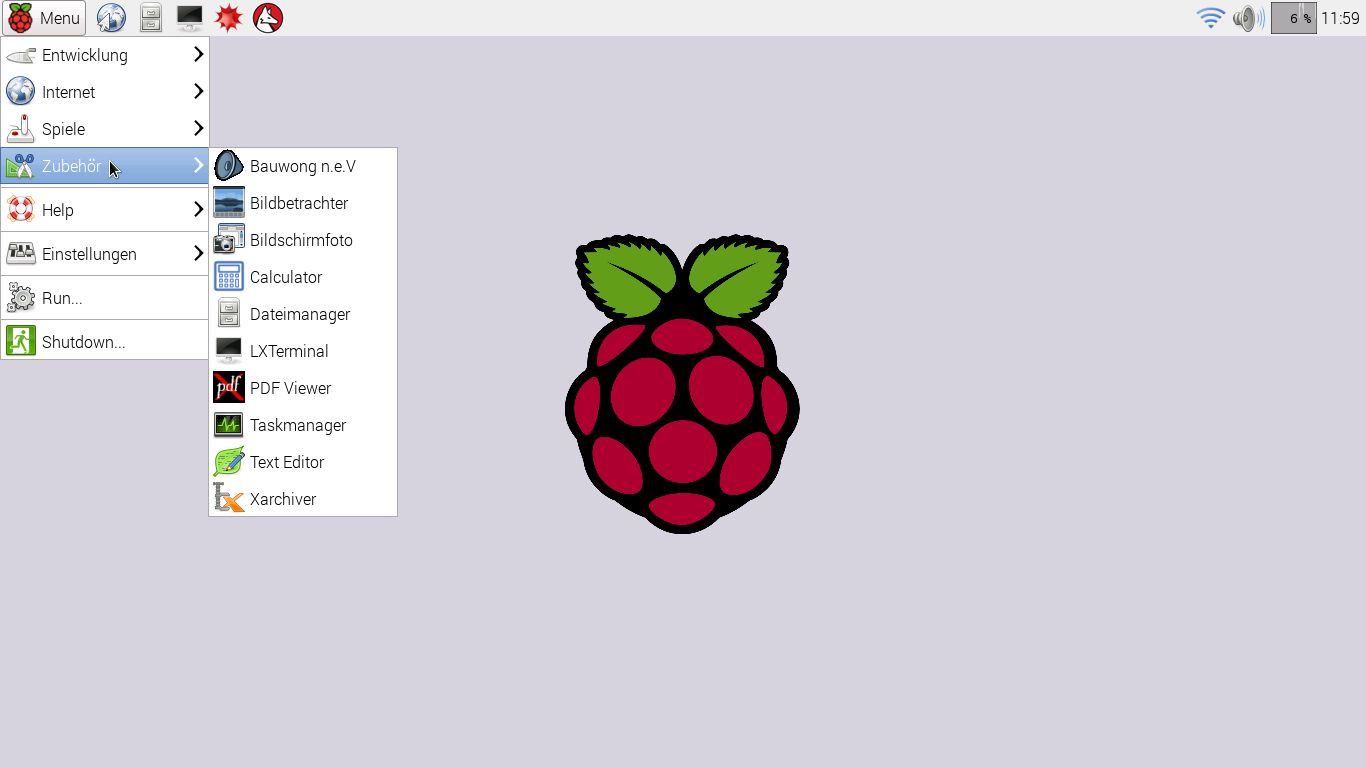
\includegraphics[width=0.8\textwidth]{startmenu.png}
\caption{Neuer Eintrag im Startmen� des \RPi}
\label{fig:startmenu}
\end{figure}

\begin{figure}[h]
\centering
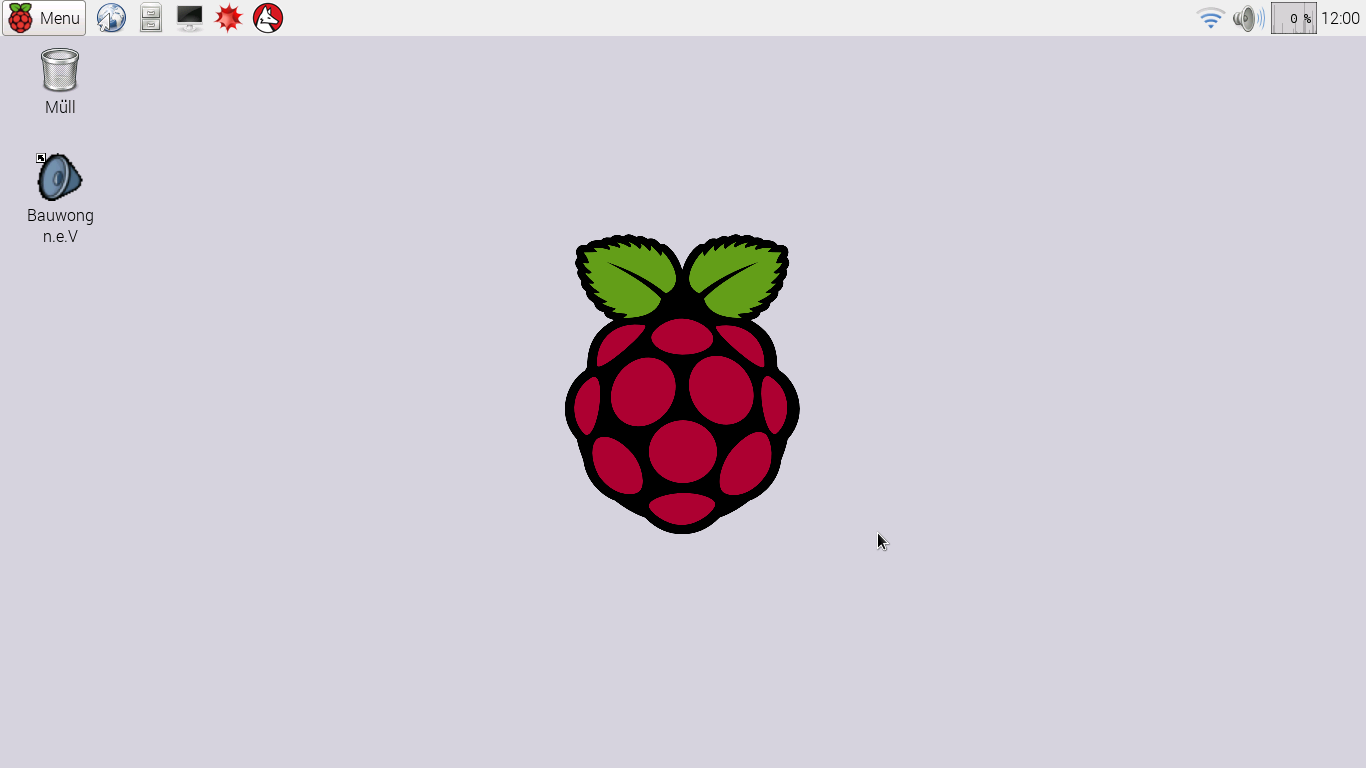
\includegraphics[width=0.8\textwidth]{desktop.png}
\caption{Neues Icon auf dem Desktop des \RPi}
\label{fig:desktop}
\end{figure}

\begin{itemize}
\item \textbf{\Bezeichnung\ ins Startmen� aufnehmen}\\
      \Code{sudo cp bauwong.desktop /usr/share/raspi-ui-overrides/applications}\\
      Wenn die Datei \filenam{bauwong.desktop} nicht ver�ndert wird, erscheint im Startmen� unter \textit{Zubeh�r} der Eintrag \textit{Bauwong n.e.V.}, siehe Abbildung \ref{fig:startmenu}.
\item \textbf{Auf dem Desktop ein Icon f�r \Bezeichnung\ anlegen}\\
      Durch Erstellung eines symbolischen Links auf die Datei \filenam[bauwong.desktop} wird ein Desktop-Icon angelegt. Dieses Icon wird sofort sichtbar, siehe Abbildung \ref{fig:desktop}.\\
      \Code{cd /home/pi/Desktop}\\
      \Code{ln -s /usr/share/raspi-ui-overrides/applications/bauwong.desktop}
\item \textbf{Autostart von \Bezeichnung\ einrichten}\\
      \Code{cd /home/pi/.config}\\
      \Code{mkdir autostart} \# falls dieses Verzeichnis noch nicht existiert\\
      \Code{cd autostart}\\
      \Code{ln -s /usr/share/raspi-ui-overrides/applications/bauwong.desktop}
\item \textbf{Bildschirmschoner des \RPi\ ausschalten}\\
      In der Datei \filenam{/etc/lightdm/lightdm.conf} muss folgende �nderung vorgenommen werden:\\
      \Code{sudo nano /etc/lightdm/lightdm.conf}
      \begin{figure}[h]
      \centering
      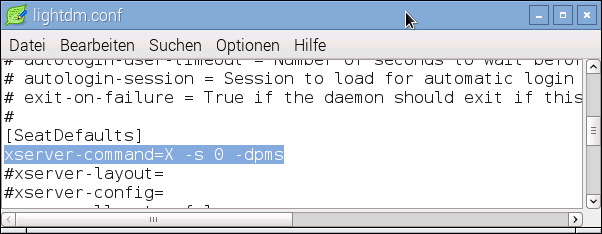
\includegraphics[width=0.6\textwidth]{screensaver.png}
      \caption{Bildschirmschoner in Datei \filenam{/etc/lightdm/lightdm.conf} deaktivieren}
      \label{fig:screensaver}
      \end{figure}
\end{itemize}


\subsection{Touchpanel-Tastatur \textit{\matchboxKeyboard} installieren}
In diesem Abschnitt wird die Installation der virtuellen Touchpanel-Tastatur\\
\textit{\matchboxKeyboard} beschrieben. Das Vorgehen wurde weitestgehend von\\
\url{http://ozzmaker.com/virtual-keyboard-for-the-raspberry-pi} �bernommen.

\begin{itemize}
\item \textbf{Compilierung von \textit{\matchboxKeyboard} vorbereiten}\\
      Softwarepakete f�r die Compilierung installieren:\\
      \Code{sudo apt-get install libfakekey-dev libpng-dev libxft-dev autoconf libtool -y}
\item \textbf{\textit{\matchboxKeyboard} compilieren}\\
      \Code{git clone https://github.com/mwilliams03/matchbox-keyboard.git}\\
      \Code{cd matchbox-keyboard}\\
      \Code{./autogen.sh}\\
      \Code{make}\\
      \Code{sudo make install}
\item \textbf{shared libraries \textit{erst nach} der Compilierung installieren!}\\
      \Code{sudo apt-get install libmatchbox1 -y}
\item \textbf{Icon \texit{Toggle Matchbox Keyboard} in der Schnellstartleiste erstellen}\\
      \Code{cd /home/pi/bauwong/keyboard}\\
      Eintrag im Startmen� unter \textit{Zubeh�r}:\\
      \Code{sudo cp matchbox-keyboard.sh /usr/local/bin}\\
      \Code{sudo chmod a+x /usr/local/bin/matchbox-keyboard.sh}\\
      \Code{sudo cp matchbox-keyboard.desktop /usr/local/share/applications/inputmethods}\\
      Shellscript \filenam{toggle-matchbox-keyboard.sh} hinzuf�gen:\\
      \Code{sudo cp toggle-matchbox-keyboard.sh /usr/bin}\\
      \Code{sudo chmod a+x /usr/bin/toggle-matchbox-keyboard.sh}\\
      \Code{sudo cp toggle-matchbox-keyboard.desktop /usr/share/applications}\\
      Eintrag des Shellscripts \filenam{toggle-matchbox-keyboard.sh} in der Schnellstartleiste:\\
      \Code{cp panel /home/pi/.config/lxpanel/LXDE-pi/panels}\\
      Die kopierte Datei \filenam{panel} entspricht dem Original mit folgender Erg�nzung:
      \begin{figure}[h]
      \centering
      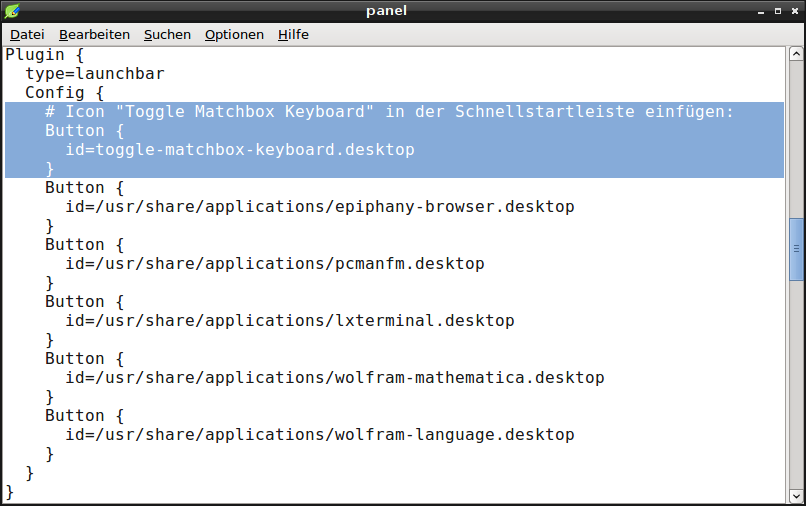
\includegraphics[width=0.7\textwidth]{launchbar.png}
      \caption{�nderungen in der Datei \filenam{/home/pi/.config/lxpanel/LXDE-pi/panels/panel}}
      \label{fig:launchbar}
      \end{figure}
      Im Abschnitt \textit{Plugin\{ Config\{ type=launchbar \} \}} m�ssen die markierten Zeilen aus Abbildung \ref{fig:launchbar} erg�nzt werden.
\item \textbf{Tastaturlayout}\\
      Ein passendes Tastaturlayout befindet sich in der Datei\\ \filenam{/home/pi/bauwong/keyboard/keyboard-bauwong.xml}. Dieses Layout kann nat�rlich noch angepasst werden. Nach der �nderung muss es nach \filenam{/usr/local/share/matchbox-keyboard} kopiert werden:\\
      \Code{sudo cp keyboard-bauwong.xml /usr/local/share/matchbox-keyboard}
\end{itemize}


\section{Erweiterungen und Verbesserungen der Software}
\label{sect:Erweiterungen}
Zuletzt noch eine Liste von Punkten, um die die Software \Bezeichnung\ erg�nzt
werden k�nnte. Hier handelt es sich um ein \textit{Brainstorming}. Die
Reihenfolge soll keine Gewichtung darstellen!

\subsection{Bedienung und grafische Oberfl�che}
\begin{itemize}
\item \textbf{Scrolling durch Wischgesten wie an einem Smartphone}\\
      horizontal und vertikal: \Code{Treeview.xview} bzw. \Code{Treeview.yview}
\item \textbf{Anzeige von Titlenummer und aktueller Laufzeit}\\
      wie bei den meisten klassischen CD-Spielern
\item \textbf{Auf die Gesamtdauer eines St�ckes skalierter "`Fortschrittsbalken"'}\\
      einfache Verschiebem�glichkeit mit Zeitanzeige wie bei den meisten Mediaplayern
\item \textbf{\textit{Drag + Drop} von Mediendateien aus der Baumstruktur in die Playlist}\\
      Damit h�tte man die M�glichkeit, neue Titel irgendwo in der Mitte der
      bestehenden Playlist einzuf�gen. Momentan werden alle neuen Titel hinten
      angeh�ngt.
\item \textbf{evtl "`Cursortasten"' f�r die Baumansicht und <ENTER> zum Aktivieren}\\
      Ist dieses Thema mit der virtuellen Tastatur erschlagen?
\end{itemize}

\subsection{Funktionalit�t von \Bezeichnung}
\begin{itemize}
\item \textbf{Anpassen auf unterschiedliche Displaygr��en}\\
      Derzeit ist eine Displaygr��e von mindestens 1366x768 Pixeln notwendig,
      da die Fenster\textbf{h�he} im Code derzeit fest eingestellt ist. Die
      Fensterbreite ist unkritischer.\\
      * Fenstergr��e flexibler programmieren!\\
      * Schriftgr��e vor allem f�rs Treeview-Steuerelement parametrierbar machen\\
      * Alles in einer config-Datei ablegen
\item \textbf{Erkennung anderer USB-Ger�tetypen (Smartphones)}\\
      Derzeit wird nur der USB-Ger�tetyp "`Mass Storage Device"' unterst�tzt.
      Viele neuere Smartphones stellen ihre Daten mitunter nur noch �ber MTP
      (Media Transfer Protocol), eine Weiterentwicklung von PTP (Picture
      Transfer Protocol) zur Verf�gung.
\item \textbf{Einbinden der vorhandenen Dateien in die Baumansicht}\\
      Derzeit wird ein USB-Laufwerk, nachdem es erkannt wurde, immer
      \textbf{komplett} (rekursiv) eingelesen! Dies kann bei gro�en Laufwerken
      mit vielen Einzeldateien mitunter recht lange dauern! Besser w�re es, nur
      das gerade ge�ffnete Verzeichnis \textbf{flach} und nicht rekursiv
      einzulesen. �ber dieses Vorgehen werden die Dateien st�ckweise registriert
      und der Vorgang dauert nie arg lange.\\
      Zu ber�cksichtigen ist das aber bei der Dateisuche, da zum Suchzeitpunkt
      nicht zwingend schon alle Unterverzeichnisse komplett eingelesen wurden!
\item \textbf{Dateitypen ber�cksichtigen}\\
      Derzeit werden alle vorhandenen Dateien angezeigt. �ber die Dateiendung oder
      eine "`magische Dateinummer"' am Dateianfang nur die Mediendateien auflisten.\\
      * Kl�ren, welche Dateitypen von \filenam{omxplayer.bin} �berhaupt unterst�tzt werden.\\
      * Playlists (\filenam{*.mpu}), Bilddateien, Textdateien, und pdf ber�cksichtigen?
\item \textbf{\filenam{omxplayer.bin}}\\
      Der omxplayer macht ein kurzes Fading (< 1 Sekunde) beim Start einer neuen
      Musikdatei. Dies ist manchmal wirklich st�rend!
\end{itemize}

Hierbei handelt es sich um die noch nicht abgearbeiteten Punkte aus meiner
Schmierzettelsammlung. Diese Liste erhebt aber keinen Anspruch auf
Vollst�ndigkeit. \smiley{smile}\\

\texttt{schlizbaeda}


%\input{Kapitel/Kapitel4}
%\input{Kapitel/Kapitel5}
%\input{Kapitel/Kapitel6}
%\input{Kapitel/Kapitel7}
%\input{Kapitel/Kapitel8}

% ##############################################################################
% ------------------------------------------------------------------------------
% ##############################################################################


% ANHANG -----------------------------------------------------------------------
%   Die Inhalte des Anhangs werden analog zu den Kapiteln inkludiert.
%   Dies geschieht in der Datei "Anhang.tex".
% ------------------------------------------------------------------------------
%\begin{appendix}
%    \clearpage
%    \pagenumbering{roman}
%    \chapter{Anhang}
%    \label{sec:Anhang}
%    % Rand der Aufz�hlungen in Tabellen anpassen
%    \setdefaultleftmargin{1em}{}{}{}{}{}
%    \begin{itemize}
%\item	Abk�rzungsverzeichnis
\item	Schaltplan
\item	St�ckliste
\end{itemize}

%%---------------------------------------------------------------
%%  Abk�rzungsverzeichnis
%%---------------------------------------------------------------
%\section{Abk�rzungsverzeichnis}
%Folgende Abk�rzungen werden im Dokument verwendet
%
%\begin{table}[!h]
%\centering
%\renewcommand{\arraystretch}{2}
%\begin{tabular}{|l|l|}
%\hline
%Sepp	&	Sepperl\\
%\hline
%Meldung	&	ndfioshoi\\
%\hline
%Meldung	&	ndfioshoi\\
%\hline
%\end{tabular}
%\vspace{0.5cm}
%\caption{Abk�rzungsverzeichnis}
%\end{table}


%---------------------------------------------------------------
%  Schaltplan
%---------------------------------------------------------------
\includepdf[pages=-, portrait, scale=1.0, addtotoc={1,section,0,Schaltplan,Schaltplan} ]{./Bilder/Anhang/Schaltplan_S1-2.pdf}
\includepdf[pages=-, portrait, scale=1.0, addtotoc={0,section,0,Schaltplan,Schaltplan} ]{./Bilder/Anhang/Schaltplan_S3.pdf}
\includepdf[pages=-, portrait, scale=1.0, addtotoc={0,section,0,Schaltplan,Schaltplan} ]{./Bilder/Anhang/Schaltplan_S4ff.pdf}

%---------------------------------------------------------------
%  St�ckliste
%---------------------------------------------------------------
\includepdf[pages=-, portrait, scale=1.0, addtotoc={1,section,0,St�ckliste,St�ckliste} ]{./Bilder/Anhang/Stueli.pdf}

%%---------------------------------------------------------------
%%  Zuweisung einer IP-Adresse an ein XPort-Modul
%%---------------------------------------------------------------
%\includepdf[pages=-, portrait, scale=1.0, addtotoc={1,section,0,IP-Zuweisung an XPort,IP-Zuweisung an XPort} ]{./Bilder/Anhang/Stueli.pdf}




%\end{appendix}

% Index ------------------------------------------------------------------------
%   Zum Erstellen eines Index, die folgende Zeile auskommentieren.
% ------------------------------------------------------------------------------
%\printindex

\end{document}
